\section*{ÔN TẬP CHƯƠNG V}
\subsection{Bài tập tự luận}
%%==========Bài 1
\begin{bt}
	\immini{
	Quan sát hình bên. Biết $\widehat{DOA}=120^{\circ}, OA \perp OC, OB \perp OD$.
	\begin{enumerate}
	\item Đọc tên các góc ở tâm có trong hình.
	\item Tính số đo của mỗi góc ở tâm tìm được ở câu a).
	\item Tìm các cặp cung bằng nhau và có số đo nhỏ hơn $180^{\circ}$.
	\item So sánh hai cung nhỏ $\wideparen{AB}$ và $\wideparen{CD}$.	
	\end{enumerate}	
	}{
	\begin{tikzpicture}[>=stealth,line join=round,line cap=round,font=\footnotesize,scale=1]
	\tikzset{declare function={r=1.5;}}
	\path 
	(0,0)coordinate (O)+(0:r)coordinate(A)+(120:r)coordinate (D)
	($(O)!{sin(90)*1}!{90}:(A)$)coordinate (C)
	($(O)!{sin(90)*1}!-{90}:(D)$)coordinate (B) 
	;
	\draw (O)circle(r);
	\foreach \pointo/\pointt in {O/A,O/B,O/C,O/D}{
	\draw[fill=black](\pointo)--(\pointt);
	}
	\foreach \point/\goc in {O/-90,A/-10,B/30,C/90,D/120}{
	\draw[fill=black](\point)circle(.8pt)+(\goc:2mm)node[scale=.8]{$\point$};
	}
	\end{tikzpicture}	
	}	
	\loigiai{
	\begin{enumerate}
	\item Các góc ở tâm có trong hình là $\widehat{AOB}$, $\widehat{AOC}$, $\widehat{AOD}$, $\widehat{BOC}$, $\widehat{BOD}$, $\widehat{COD}$.
	\item Ta có $OA \perp OC$, $OB \perp OD$ nên $\widehat{AOC}=90^{\circ}$, $\widehat{BOD}=90^{\circ}$.	\\
	Khi đó $\widehat{AOB}=\widehat{AOD}-\widehat{BOD}=120^{\circ}-90^{\circ}=30^{\circ}$,\\ $\widehat{COD}=\widehat{AOD}-\widehat{AOC}=120^{\circ}-90^{\circ}=30^{\circ}$,\\
	$\widehat{BOC}=\widehat{AOC}-\widehat{AOB}=90^{\circ}-30^{\circ}=60^{\circ}$.
	\item Ta có 
	$\widehat{AOC}=\widehat{BOD}\Rightarrow \wideparen{AC}=\wideparen{BD}$;	\\ $\widehat{AOB}=\widehat{DOC}\Rightarrow \wideparen{AB}=\wideparen{CD}$;
	\item Ta thấy $\wideparen{AB}=\wideparen{CD}$.
	\end{enumerate}
	}
\end{bt}
%%==========Bài 2
\begin{bt}
	Chứng minh trong một đường tròn:
	\begin{enumerate}
	\item Đường kính vuông góc với một dây thì đi qua trung điểm của dây ấy;
	\item Đường kính đi qua trung điểm của một dây không đi qua tâm thì vuông góc với dây ấy;
	\item Hai dây bằng nhau thì cách đều tâm;
	\item Hai dây cách đều tâm thì bằng nhau.
	\end{enumerate}
	\loigiai{
	\immini{
	\begin{enumerate}
	\item Giả sử đường kính $MN$ vuông góc với dây $AB$ tại $I$.\\
	Khi đó $\triangle OIA=\triangle OIB$ (c-g-c). Suy ra $IA=IB$ hay $I$ là trung điểm của $AB$.
	\item Giả sử đường kính $MN$ đi qua trung điểm $I$ của dây không đi qua tâm $AB$.\\
	Khi đó $\triangle OIA=\triangle OIB$ (c-c-c). Suy ra $\widehat{OIA}=\widehat{OIB}=90^\circ$ hay $OI\perp AB$.
	\item Cho hai dây $AB=CD$. Gọi $I,K$ lần lượt là hình chiếu của $O$ trên $AB,CD$.\\
	Khi đó ta có $IA=IB=KC=KD$. Sử dụng tam giác bằng nhau suy ra $OI=OK$ hay hai dây cách đều tâm.
	\end{enumerate}
	}{
	\begin{tikzpicture}[font=\scriptsize,scale=0.85]
	\def\r{3}
	\coordinate (O) at (0,0);
	\coordinate (A) at (-30:\r);
	\coordinate (B) at (210:\r);
	\coordinate (C) at (30:\r);
	\coordinate (D) at (150:\r);
	\coordinate (K) at ($(C)!1/2!(D)$);
	\coordinate (M) at (90:\r);
	\coordinate (N) at (-90:\r);
	\coordinate (I) at ($(A)!1/2!(B)$);
	\draw(O) circle (\r);
	\draw(A)--(B)(M)--(N)(C)--(D)(O)--(A)(O)--(B)(C)--(O)--(D);
	\foreach \p/\g in {O/0,A/0,B/180,I/45, C/0, D/180, K/45, M/90, N/-90}\draw[fill=black] (\p) circle (1pt)node[shift={(\g:.3)},scale=1]{$\p$};
	\end{tikzpicture}
	}
	\begin{enumerate}\setcounter{enumi}{3}
	\item Cho hai dây $AB,CD$ có $I,K$ lần lượt là hình chiếu của $O$ trên $AB,CD$ và $OI=OK$. Sử dụng tam giác bằng nhau ta có $IA=IB=KC=KD$ hay $AB=CD$.
	\end{enumerate}
	}
\end{bt}
%%==========Bài 3
\begin{bt}
	Cho $AB$ là một dây bất kì (không phải là đường kính) của đường tròn $(O; 4 \mathrm{cm})$. Gọi $C$ và $D$ lần lượt là các điểm đối xứng với $A$ và $B$ qua tâm $O$.
	\begin{listEX}[1]
	\item Hai điểm $C$ và $D$ có nằm trên đường tròn $(O)$ không? Vì sao?
	\item Biết rằng $ABCD$ là một hình vuông. Tính độ dài cung lớn $AB$ và diện tích hình quạt tròn tạo bởi hai bán kính $OA$ và $OB$.
	\end{listEX}
	\loigiai{
	\immini{
	\begin{listEX}[1]
	\item Vì $C$ và $D$ lần lượt là các điểm đối xứng với $A$ và $B$ qua tâm $O$ nên\\
	$\heva{&OA=OC\\&OB=OD}\Rightarrow OA=OB=OC=OD$.\\
	$ \Rightarrow A,B,C,D$ cách đều $O$.\\ 
	Suy ra hai điểm $C$ và $D$ có nằm trên đường tròn $(O)$.
	\item Vì $ABCD$ là hình vuông nên $\Delta ABO$ là tam giác vuông cân tại $O$.\\
	Áp dụng định lý Pythagore vào tam giác $ABO$ vuông tại $O$ có\\ $AB=\sqrt{AO^2+OB^2}=\sqrt{4^2+4^2}=4\sqrt{2}$ (cm).\\
	Độ dài cung lớn $AB$ là $l=\dfrac{360-90}{360}\cdot\pi\cdot 4=3\pi$ (cm).
	\\ Diện tích hình quạt tròn tạo bởi hai bán kính $OA$ và $OB$ là $S_q=\dfrac{90}{360}\cdot\pi \cdot 4^2=4\pi$ (cm$^2$).
	\end{listEX}}{
	\begin{tikzpicture}[>=stealth,line join=round,line cap=round,font=\footnotesize,scale=1]
	\def\r{2cm}
	\path 
	(0,0) coordinate (O)
	(45:\r) coordinate (B)
	(135:\r) coordinate (A)
	($(A)!2!(O)$) coordinate (C)
	($(B)!2!(O)$) coordinate (D);	
	\draw 
	(O) circle (\r)
	(A)--(B)--(C)--(D)--cycle;
	\draw[dashed] (A)--(O)node[midway, left]{$4$}--(C) (B)--(D);
	\foreach \m/\n in{O/90,A/180,B/0,C/0,D/180}
	\fill[black] (\m) circle(1.5pt)+(\n:3mm)node{$\m$};
	\end{tikzpicture}
	}}
\end{bt}
%%==========Bài 4
\begin{bt}
	Hãy hoàn thành bảng số liệu sau vào vở (lấy $\pi=3{,}14$ và làm tròn kết quả đến hàng phần mười).
	\begin{center}
	\begin{tabular}{|c|c|c|c|c|c|}
	\hline
	Bán kính $R$ & $20\,\text{cm}$ & $?$ & $12\,\text{cm}$ & $32{,}6\,\text{cm}$ & $?$ \\
	\hline
	Số đo $n^{\circ}$ của cung tròn &$160^{\circ}$ & $144^{\circ}$ & $?$ & $42^{\circ}$ & $15^{\circ}$ \\
	\hline
	Độ dài $l$ của cung tròn & $?$ & $16{,}8\,\text{cm}$ & $60\,\text{cm}$ & $?$ & $96\,\text{cm}$ \\
	\hline
	\end{tabular}
	\end{center}	
	\loigiai{
	\begin{center}
	\begin{tabular}{|c|c|c|c|c|c|}
	\hline
	Bán kính $R$ & $20\,\text{cm}$ & $6{,}7\,\text{cm}$ & $12\,\text{cm}$ & $32{,}6\,\text{cm}$ & $366{,}8\,\text{cm}$ \\
	\hline
	Số đo $n^{\circ}$ của cung tròn &$160^{\circ}$ & $144^{\circ}$ & $286{,}6^{\circ}$ & $42^{\circ}$ & $15^{\circ}$ \\
	\hline
	Độ dài $l$ của cung tròn & $55{,}8\,\text{cm}$ & $16{,}8\,\text{cm}$ & $60\,\text{cm}$ & $23{,}9\,\text{cm}$ & $96\,\text{cm}$ \\
	\hline
	\end{tabular}
	\end{center}	
	}
\end{bt}
%%==========Bài 5
\begin{bt}
	\immini{
	Logo ở hình bên có dạng một hình quạt tròn bán kính $8$cm và góc ở tâm bằng $60^\circ$. Tính diện tích mỗi hình sau (theo đơn vị centimét vuông và làm tròn kết quả đến hàng phần mười):
	\begin{enumerate}
	\item Toàn bộ logo;
	\item Phần logo màu đỏ có dạng hình viên phân.
	\end{enumerate}
	}{
	\begin{tikzpicture}[scale=.4]
	\coordinate (O) at (0,0);
	\coordinate (B) at ($(O)+(60:8)$);
	\draw[fill=red, thick] (B) arc (60:120:8) coordinate (A)--(B);
	\draw(B)--(O)--(A)--(B);
	\end{tikzpicture}
	}
	\loigiai{
	\begin{enumerate}
	\item Diện tích toàn bộ logo là $S_1=\dfrac{\pi\cdot8^2\cdot60}{360}=10{,}67\cdot3{,}14=33{,}5$ (cm$^2$).
	\item Diện tích tam giác là $S_2=\dfrac{8^2\sqrt3}{4}=27{,}7$ (cm$^2$).\\
	Suy ra diện tích phần logo màu đỏ là $S_1-S_2=5{,}8$ (cm$^2$).
	\end{enumerate}
	}
\end{bt}
%%==========Bài 6
\begin{bt}
	\immini{
	Hình bên biểu diễn vùng biển được chiếu sáng bởi một hải đăng có dạng một hình quạt tròn với bán ính $18$ dặm, cung $AmB$ có số đo $245^\circ$.
	\begin{enumerate}
	\item Hãy tính diện tích vùng biển có thể nhìn thấy ánh sáng từ hải đăng theo đơn vị kilômét vuông (lấy $1$ dặm $=1~600$m, $\pi=3{,}14$ và làm tròn kết quả đến hàng đơn vị).
	\item Giả sử một con thuyền di chuyển dọc theo dây cung có độ dài $28$ dặm của đường tròn với tâm là tâm của hình quạt tròn, bán kính là $18$ dặm. Tính khoảng cách nhỏ nhất từ con thuyền đến hải đăng (theo đơn vị dặm và làm tròn kết quả đến hàng đơn vị).
	\end{enumerate}
	}{
	\begin{tikzpicture}[font=\scriptsize,scale=0.85]
	\def\r{3.6}
	\coordinate (O) at (0,0);
	\coordinate (B) at ($(-45:\r)$);
	\coordinate (A) at ($(225:\r)$);
	\coordinate (H) at ($(O)+(0,-.3)$);
	\coordinate (C) at (30:\r);
	\coordinate (D) at (150:\r);
	\draw(C)--(D)node[midway, below]{$28$ dặm}node[midway, shift={(1,.1)}]{\twemoji[height=.5cm]{26f4}};
	\draw (H) circle (.2)node[below, shift={(0,-.3)}]{Hải đăng};
	\draw (O)--(B)node[midway, right]{$18$ dặm} arc (-45:225:\r)--(A)--(O);
	\foreach \p/\g in {A/-90,B/-90}\draw[fill=black] (\p) circle (1pt)node[shift={(\g:.3)},scale=1]{$\p$};
	%	\draw(-4,-4)--(-4,4)--(4,4)--(4,-4)--(-4,-4);
	\end{tikzpicture}
	}
	\loigiai{
	Đổi $18$ dặm $=28{,}8$ km; $28$ dặm $=44{,}8$ km.
	\begin{enumerate}
	\item Diện tích vùng biển có thể nhìn thấy ánh sáng từ hải đăng là 
	\begin{center}
	$\dfrac{\pi\cdot28{,}8^2\cdot245}{360}=1~722{,}5$ (km$^2$).
	\end{center}
	\item Khoảng cách nhỏ nhất từ con thuyền đến ngọn hải đăng là khoảng cách từ tâm đến dây cung và bằng $\sqrt{18^2-\left(\dfrac{28}2\right)^2}=\sqrt{128}=11{,}3$ (dặm).
	\end{enumerate}
	}
\end{bt}
%%==========Bài 7
\begin{bt}
	\immini{
	Mặt đĩa CD ở hình bên có dạng hình vành khuyên giới hạn bởi hai đường tròn có bán kính lần lượt là $1{,}5$cm và $6$cm. Hình vành khuyên đó có diện tích bằng bao nhiêu centimét vuông (làm tròn kết quả đến hàng phần mười)?
	}{
	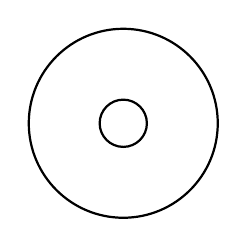
\begin{tikzpicture}[scale=.2]
	\coordinate (O) at (0,0);
	\draw[thick] (O) circle (1.5);
	\draw[thick] (O) circle (6);
	\end{tikzpicture}
	}
	\loigiai{
	Diện tích đường tròn to là $S_1=\pi\cdot6^2=36\pi$ (cm$^2$).\\
	Diện tích đường tròn nhỏ là $S_2=\pi\cdot1{,}5^2=2{,}25\pi$ (cm$^2$).\\
	Diện tích hình vành khuyên là $S_1-S_2=(36-2{,}25)\pi=33{,}75\cdot3{,}14\approx106$ (cm$^2$).
	}
\end{bt}
%%==========Bài 8
\begin{bt}
	\immini{
	Hình bên mô tả mảnh vải có dạng một phần tư hình vành khuyên, trong đó hình vành khuyên giới hạn bởi hai đường tròn cùng tâm và có các bán kính lần lượt là $3$dm và $5$dm. Diện tích của mảnh vải đó bằng bao nhiêu decimét vuông (làm tròn kết quả đến hàng phần mười)?
	}{
	\begin{tikzpicture}[scale=.4]
	\coordinate (O) at (0,0);
	\coordinate (B) at ($(O)+(45:3)$);
	\coordinate (D) at ($(O)+(45:5)$);
	\draw[thick] (B) arc (45:135:3) coordinate (A);
	\draw[thick] (D) arc (45:135:5) coordinate (C);
	\draw[thick](A)--(C)(B)--(D);
	\draw[dashed](O)--(B)(O)--(A);
	\foreach \i/\j/\k/\t in {O/A/B/12}{
	\def\dgiua{\i}\def\dmot{\j}\def\dhai{\k}\def\tyso{\t pt}
	\draw ($(\dgiua)!\tyso!(\dmot)$)--($(\dgiua)!2!($($(\dgiua)!\tyso!(\dmot)$)!.5!($(\dgiua)!\tyso!(\dhai)$)$)$)--($(\dgiua)!\tyso!(\dhai)$);}
	\end{tikzpicture}
	}
	\loigiai{
	Diện tích hình quạt to là $S_1=\dfrac{\pi\cdot5^2\cdot90}{360}=6{,}25\pi$ (dm$^2$).\\
	Diện tích hình quạt nhỏ là $S_2=\dfrac{\pi\cdot3^2\cdot90}{360}=2{,}25\pi$ (dm$^2$).\\
	Diện tích mảnh vải là $S_1-S_2=(6{,}25-2{,25})\pi=4\cdot3{,}14=12{,}6$ (dm$^2$).
	}
\end{bt}
%%==========Bài 9
\begin{bt}
	Hải đăng Kê Gà tọa lạc tại xã Tân Thanh huyện Hàm Thuận Năm, tỉnh Bình Thuận. Biết ngọn hải đăng cao $65$ m so với mực nước biển. Với khoảng cách bao nhiêu kilômét thì người quan sát trên tàu bắt đầu trông thấy ngọn hải đăng này? Cho biết mắt người quan sát ở độ cao $5$ m so với mực nước biển và bán kính Trái Đất gần bằng $6\,400$ km.
	\begin{center}
	\includegraphics[scale=1.2]{images/ON-TAP-C5-SGK-9-CTST-T1-cau-15}
	\begin{tikzpicture}[>=stealth,line join=round,line cap=round,font=\footnotesize,scale=1]
	\tikzset{declare function={r=1.5;}}
	\draw (0,0)coordinate (O) circle (r);
	\path 
	($(O)+(46:r)$) coordinate (H)
	($(H)!{sin(90)*1}!-{90}:(O)$)coordinate (A)
	($(A)!1.5!(H)$)coordinate (B)
	($(B)!.1!(O)$)coordinate (a)
	($(A)!.2!(O)$)coordinate (b)
	pic[draw,angle radius=2mm]{right angle =O--H--A}
	;
	\foreach \pointo/\pointt in {O/H,H/A,O/A,O/B,B/H}{
	\draw[fill=black](\pointo)--(\pointt);
	}
	\path 
	(A)--(b)node[left,scale=.8]{$65$ m}
	(B)--(a)node[below right,scale=.8]{$5$ m}
	;
	\foreach \point/\goc in {O/-90,H/65,A/90,B/20}{
	\draw[fill=black](\point)circle(.2pt)+(\goc:2mm)node[scale=.8]{$\point$};}
	\end{tikzpicture}
	\end{center}
	\loigiai{
	Ta có $\triangle OHA$ và $\triangle OHB$ là các tam giác vuông tại $H$, theo định lí Pythagore\\
	$AH=\sqrt{OA^2-OH^2}=\sqrt{(6400+65\cdot 10^{-3})^2-6400^2}\approx 28{,}844 $ km.\\
	$BH=\sqrt{OB^2-OH^2}=\sqrt{(6400+5\cdot 10^{-3})^2-6400^2}\approx 8$ km.
	Khoảng cách để người quan sát trên tàu trông thấy ngọn hải đăng là $AB=AH+HB=28{,}844+8=36{,}844$ km.	
	}
\end{bt}
%%==========Bài 10
\begin{bt}
	Cho đường tròn $(O)$ đường kính $BC$ và điểm $A$ (khác $B$ và $C$).
	\begin{listEX}[1]
	\item Chứng minh rằng nếu $A$ nằm trên $(O)$ thì $ABC$ là một tam giác vuông; ngược lại, nếu $ABC$ là tam giác vuông tại $A$ thì $A$ nằm trên $(O)$.
	\item Giả sử $A$ là một trong hai giao điểm của đường tròn $(B; BO)$ với đường tròn $(O)$. Tính các góc của tam giác $ABC$.
	\item Với cùng giả thiết câu b, tính độ dài cung $AC$ và diện tích hình quạt nằm trong $(O)$ giới hạn bởi các bán kính $OA$ và $OC$, biết rằng $BC=6 \mathrm{cm}$.
	\end{listEX}
	\loigiai{
	\begin{listEX}[1]
	\item Xét tam giác $ABC$ nội tiếp đường tròn $O$ đường kính $BC$, ta có:
	$OA=OB=OC$.
	\immini{
	Tam giác $ABC$ có đường trung tuyến $AO$ bằng nửa cạnh $BC$ nên suy ra tam giác $ABC$ vuông tại $A$. (đpcm)
	\\Vì tam giác $ABC$ vuông tại $A$, theo tính chất đường trung tuyến ứng với cạnh huyền trong tam giác vuông, ta có
	\[OA=OB=OC\]
	Suy ra $O$ cách đều $A$, $B$, $C$. Hay $A$, $B$, $C$ thuộc đường tròn tâm $O$. Nói cách khác thì $A$ nằm trên $(O)$. (đpcm)
	}{
	\begin{tikzpicture}[>=stealth,line join=round,line cap=round,font=\footnotesize,scale=1]
	\def\r{2cm}
	\path 
	(0,0) coordinate (O)
	(50:\r) coordinate (A)
	(0:\r) coordinate (C)
	(-180:\r) coordinate (B);	
	\draw 
	(O) circle (\r)
	(B)--(C)--(A)--cycle (O)--(A);
	\pic[draw,angle radius=0.2cm]{right angle=B--A--C};
	\foreach \m/\n in{A/50,O/-90,B/180,C/0}
	\fill[black] (\m) circle(1.5pt)+(\n:3mm)node{$\m$};
	\end{tikzpicture}}
	\item Vì $O$, $A$ nằm trên $(B,BO)$ suy ra $BO=BA$. \quad(1)\\
	Vì $A$, $B$ nằm trên $(O,AO)$ suy ra $$\heva{&OB=OA&(2)\\&\widehat{BAO}=90^{\circ}.&(\text{theo câu a})}$$
	Từ (1) và (2) suy ra\\
	$OA=OB=AB\Rightarrow \Delta ABO$ đều.\\
	$\Rightarrow \widehat{ABO}=60^{\circ}.$
	\immini{
	Xét $\Delta ABC$ ta có
	\begin{align*}
	&\widehat{ABC}+\widehat{ACB}+\widehat{BAC}=180^{\circ}\\
	\Rightarrow& \widehat{ACB}=180^{\circ}-\widehat{ABC}-\widehat{BAC}\\
	\Rightarrow&\widehat{ACB}=180^{\circ}-60^{\circ}-90^{\circ}=30^{\circ}.
	\end{align*} 
	\item 
	Bán kính đường tròn tâm $O$ là $R=\dfrac{BC}{2}=\dfrac{6}{2}=3$ (cm).\\
	Suy ra độ dài $l$ của cung $AC$ là $l=\dfrac{60}{180}\cdot \pi\cdot 3=\pi$ (cm).
	\\Ta có $\widehat{AOC}=180^{\circ}-\widehat{AOB}=180^{\circ}-60^{\circ}=120^{\circ}$\quad (do $\triangle ABO$ đều).\\
	Suy ra diện tích hình quạt cần tính là $S_q=\dfrac{120}{360} \cdot\pi\cdot 3^2=3\pi$ (cm$^2$).
	}{
	\begin{tikzpicture}[>=stealth,line join=round,line cap=round,font=\footnotesize,scale=1]
	\def\r{2.5cm}
	\path 
	(0,0) coordinate (O)
	(0:\r) coordinate (C)
	(-180:\r) coordinate (B);	
	\draw[name path=c1](O) circle (\r);
	\draw[name path=c2](B) circle (\r);
	\path [name intersections={of=c1 and c2,by={A}}];
	\draw (A)--(B)--(C)--(A)--(O);
	\foreach \m/\n in{A/90,O/-60,B/180,C/0}
	\fill[black] (\m) circle(1.5pt)+(\n:3mm)node{$\m$};
\end{tikzpicture}}
	\end{listEX}
	}
\end{bt}
%%==========Bài 11
\begin{bt}
	Cho điểm $B$ nằm giữa hai điểm $A$ và $C$, sao cho $AB=2 \mathrm{cm}$ và $BC=1 \mathrm{cm}$. Vẽ các đường tròn $(A; 1{,}5 \mathrm{cm})$, $(B; 3 \mathrm{cm})$ và $(C; 2 \mathrm{cm})$. Hãy xác định các cặp đường tròn:
	\begin{listEX}[3]
	\item Cắt nhau;
	\item Không giao nhau;
	\item Tiếp xúc với nhau.
	\end{listEX}
	\loigiai{
	\immini{
	\begin{listEX}[1]
	\item $(A; 1{,}5 \mathrm{cm})$ với $(B; 3 \mathrm{cm})$, $(A; 1{,}5 \mathrm{cm})$ với $(C; 2 \mathrm{cm})$.
	\item Không có.
	\item $(B; 3 \mathrm{cm})$ với $(C; 2 \mathrm{cm})$.
	\end{listEX}}{
	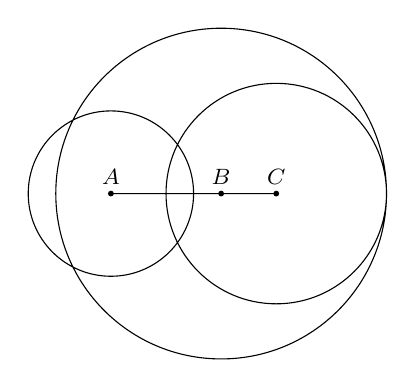
\begin{tikzpicture}[>=stealth,line join=round,line cap=round,font=\footnotesize,scale=0.7]
	\def\a{2cm}
	\def\b{1cm}
	\path 
	(0,0) coordinate (A)
	(0:\a) coordinate (B)
	++(0:\b) coordinate (C);
	\draw 
	(A) circle (\b*1.5)
	(B) circle (\b*3)
	(C) circle (\b*2)	
	(A)--(C);
	\foreach \m/\n in{A/90,B/90,C/90}
	\fill[black] (\m) circle(1.5pt)+(\n:3mm)node{$\m$};
	\end{tikzpicture}
	}}
\end{bt}
%%==========Bài 12
\begin{bt}
	Cho tam giác vuông $ABC$ ($\widehat{A}$ vuông). Vẽ hai đường tròn $(B; BA)$ và $(C; CA)$ cắt nhau tai $A$ và $A'$. Chứng minh rằng:
	\begin{listEX}[1]
	\item $BA$ và $BA'$ là hai tiếp tuyến cắt nhau của đường tròn $(C; CA)$.
	\item $CA$ và $CA'$ là hai tiếp tuyến cắt nhau của đường tròn $(B; BA)$.
	\end{listEX}
	\loigiai{
	\begin{listEX}[1]
	\item Xét $\triangle ABC$ và $\triangle A'BC$ có
	\begin{itemize}
	\item $AB=A'B$ (bán kính $(B)$)
	\item $CA=C'A$ (bán kính $(C)$)
	\item $BC$ chung	
	\end{itemize}
	Suy ra $\triangle ABC=\triangle A'BC$ (c-c-c).\\
	Nên $\widehat{BAC}=\widehat{BA'C}=90^{\circ}$ ($2$ góc tương ứng).\\
	Tức là 
	\begin{itemize}
	\item $BA'$ vuông góc bán kính $CA'$ tại $A'$, hay $BA'$ là tiếp tuyến của $(C)$. \hfill (1)
	\item $BA$ vuông góc bán kính $CA$ tại $A$, hay $BA$ là tiếp tuyến của $(C)$. \hfill (2)
	\end{itemize}
	\immini{
	Lại có $AC$ giao $A'C$ tại $C$. \hfill (3)\\
	Từ (1), (2) và (3) suy ra $BA$ và $BA'$ là hai tiếp tuyến cắt nhau của đường tròn $(C; CA)$.
	\item Vì $\widehat{BAC}=\widehat{BA'C}=90^{\circ}$ (chứng minh trên).
	\\
	Tức là 
	\begin{itemize}
	\item $CA'$ vuông góc bán kính $BA'$ tại $A'$, hay $CA'$ là tiếp tuyến của $(B)$. \hfill (1)
	\item $CA$ vuông góc bán kính $BA$ tại $A$, hay $CA$ là tiếp tuyến của $(B)$. \hfill (2)
	\end{itemize}
	Lại có $AB$ giao $A'B$ tại $C$. \hfill (3)\\
	Từ (1), (2) và (3) suy ra $CA$ và $CA'$ là hai tiếp tuyến cắt nhau của đường tròn $(B; BA)$.}{
	\begin{tikzpicture}[>=stealth,line join=round,line cap=round,font=\footnotesize,scale=.5]
	\def\b{3cm}
	\def\c{4cm}
	\path 
	(0,0) coordinate (A)
	(0:\b) coordinate (B)
	(90:\c) coordinate (C)
	;	
	\draw (A)--(B)--(C)--(A) ;
	\draw[name path=c1] (B) circle (\b);
	\draw[name path=c2] (C) circle (\c);
	\path [name intersections={of=c1 and c2,by={A',D}}];
	\draw (B)--(A')--(C);
	\pic[draw,angle radius=0.2cm]{right angle=B--A--C};
	\pic[draw,angle radius=0.2cm]{right angle=B--A'--C};
	\foreach \m/\n in{A/-140,B/-60,C/90,A'/45}
	\fill[black] (\m) circle(1.5pt)+(\n:5mm)node{$\m$};
	\end{tikzpicture}
	}
	\end{listEX}
	}
\end{bt}
%%==========Bài 13
\begin{bt}
	\immini{
	Cho hai đường tròn $(O)$ và $(O')$ cắt nhau tại $A$ và $B$. Một đường thẳng $d$ đi qua $A$ cắt $(O)$ tại $E$ và cắt $(O')$ tại $F(E$ và $F$ khác $A)$. Biết điểm $A$ nằm trong đoạn $E F$. Gọi $I$ và $K$ lần lượt là trung điểm của $AE$ và $AF$.
	\begin{listEX}[1]
	\item Chứng minh rằng tứ giác $OO'KI$ là một hình thang vuông.
	\item Chứng minh rằng $IK=\dfrac{1}{2}EF$.
	\item Khi $d$ ở vị trí nào ($d$ vẫn qua $A)$ thì $OO'KI$ là một hình chữ nhật?
	\end{listEX}
	}{
	\begin{tikzpicture}[>=stealth,line join=round,line cap=round,font=\footnotesize,scale=0.7]
	\def\x{3cm}
	\def\y{2cm}
	\path 
	(0,0) coordinate (O)
	++(0:\y*1.8)coordinate (O')
	(140:\x*1.4) coordinate (C);
	\draw[name path=c1] (O) circle (\x);
	\draw[name path=c2] (O') circle (\y);
	\path[name intersections={of= c1 and c2}] coordinate(A)at(intersection-1)
	coordinate(B)at(intersection-2)
	($(C)!1.6!(A)$) coordinate (D);
	\draw[name path=cd] (C)node[above right]{$d$}--(D);
	\path[name intersections={of= cd and c1}] coordinate(E)at(intersection-2);
	\path[name intersections={of= cd and c2}] coordinate(F)at(intersection-1)
	($(E)!1/2!(A)$) coordinate (I)
	($(F)!1/2!(A)$) coordinate (K);
	\draw (O)--(O')--(K)--(I)--cycle;
	\pic[draw,angle radius=0.2cm]{right angle=O--I--A};
	\pic[draw,angle radius=0.2cm]{right angle=A--K--O'};
	\foreach \m/\n in{A/90,B/-90,O/-90,O'/-90,E/90,F/30,I/80,K/80}
	\fill[black] (\m) circle(1.5pt)+(\n:3mm)node{$\m$};	
	\end{tikzpicture}	
	}
	\loigiai{
	\begin{listEX}[1]
	\item Do $\heva{&OI \perp EF\\&O'K \perp EF}\Rightarrow \heva{&OI \parallel O'K &\text{(từ vuông góc đến song song)}\\&\widehat{OIK}=90^{\circ}&}$\\
	$\Rightarrow$ tứ giác $OO'KI$ là hình thang vuông.
	\item Vì $I$ và $K$ lần lượt là trung điểm của $AE$ và $AF$ nên
	$\heva{&IA=\dfrac{1}{2}AE&(1)\\&KA=\dfrac{1}{2}AF. &(2)}$\\
	Cộng (1) và (2) theo vế ta được
	$\begin{aligned}[t]
	&IA+AK=	\dfrac{1}{2}AE+\dfrac{1}{2}AF\\
	\Rightarrow&IK=\dfrac{1}{2}(AE+AF)\\
	\Rightarrow&IK=\dfrac{1}{2}EF.
	\end{aligned}$
	\item Vì tứ giác $OO'KI$ là hình thang vuông, nên để tứ giác $OO'KI$ là hình chữ nhật thì $IK\parallel OO'$, hay $d\parallel OO'$.
	\end{listEX}
	}
\end{bt}
%%==========Bài 14
\begin{bt}
	Cho hình vuông $ABCD$ cạnh $r$ và đường tròn $(C;r)$. Giả sử $M$ là một điểm nằm trên đường tròn $(C;r)$ sao cho điểm $M$ nằm trong hình vuông $ABCD$. Tiếp tuyến của đường tròn $(C;r)$ tại tiếp điểm $M$ cắt các đoạn thẳng $AB,AD$ lần lượt tại $N,P$. Chứng minh:
	\begin{enumerate}
	\item Các đường thẳng $NB,PD$ là các tiếp tuyến của đường tròn $(C;r)$;
	\item $\widehat{NCP}=\widehat{NCB}+\widehat{PCD}=45^\circ$.
	\end{enumerate}
	\loigiai{
	\immini{
	\begin{enumerate}
	\item Vì $ABCD$ là hình vuông nên $NB\perp CB$, do đó $NB$ là tiếp tuyến của $(C;r)$.\\
	Tương tự $PD$ là tiếp tuyến của $(C;r)$.
	\item Ta có $\widehat{MCN}=\widehat{NCB}$ (tính chất hai tiếp tuyến cắt nhau).\\
	Tương tự, $\widehat{PCM}=\widehat{PCD}$.\\
	Do đó $\widehat{NCP}=\widehat{NCM}+\widehat{MCP}=\widehat{NCB}+\widehat{PCD}$.\\
	Ta lại có $\widehat{BCN}+\widehat{NCM}+\widehat{MCP}+\widehat{PCD}=90^\circ$. Do đó $\widehat{NCP}=45^\circ$.
	\end{enumerate}
	}{
	\begin{tikzpicture}[font=\scriptsize,scale=0.75]
	\def\r{3}	
	\coordinate (A) at (0,0);
	\coordinate (B) at (\r,0);
	\coordinate (C) at (\r,\r);
	\coordinate (D) at (0,\r);
	\draw ($(C)+(-140:\r)$) coordinate (M);
	\coordinate (T) at ($(M)!1!90:(C)$);
	\coordinate (T') at ($(M)!1!-90:(C)$);
	\draw(A)--(B)--(C)--(D)--(A)(C)--(M);
	\path (intersection of A--B and M--T') coordinate (N);
	\path (intersection of A--D and M--T) coordinate (P);
	\draw(C) circle (\r);
	\draw(C)--(N)--(P)--(C);
	\foreach \p/\g in {A/-90,B/-90,C/90,D/150, P/180, N/-90, M/-120}\draw[fill=black] (\p) circle (1pt)node[shift={(\g:.3)},scale=1]{$\p$};
	\foreach \i/\j/\k/\t in {A/B/D/6, B/A/C/6, D/A/C/6, M/C/N/6}{
	\def\dgiua{\i}\def\dmot{\j}\def\dhai{\k}\def\tyso{\t pt}
	\draw ($(\dgiua)!\tyso!(\dmot)$)--($(\dgiua)!2!($($(\dgiua)!\tyso!(\dmot)$)!.5!($(\dgiua)!\tyso!(\dhai)$)$)$)--($(\dgiua)!\tyso!(\dhai)$);}
	\end{tikzpicture}
	}
	}
\end{bt}
%%==========Bài 15
\begin{bt}
	Cho hai đường tròn $(I;r)$ và $(K;R)$ tiếp xúc ngoài với nhau tại $P$ với $R\ne r$, đường thẳng $a$ lần lượt tiếp xúc với $(I;r)$ và $(K;R)$ tại $A$ và $B$, $a$ cắt $KI$ tại $O$. Đường thẳng qua $P$ vuông góc với $IK$ cắt đường thẳng $a$ tại $M$. Chứng minh:
	\begin{enumEX}{3}
	\item $\dfrac{OI}{OK}=\dfrac rR$;
	\item $AB=2MP$;
	\item $\widehat{IMK}=90^\circ$.
	\end{enumEX}
	\loigiai{
	\begin{center}
	\begin{tikzpicture}[declare function={R=2;r =4;d = R+r;goc=acos((R-r)/d);},scale=0.55]
	\path 	(0,0) coordinate (I)+(d,0) coordinate (K)
	(goc:R) coordinate (A)
	($ (d,0)+(goc:r) $) coordinate (B)
	(intersection of B--A and I--K) coordinate (O)
	(0:R) coordinate (P)
	($(P)!1!-90:(I)$) coordinate (p)
	(intersection of B--A and P--p) coordinate (M);
	\draw [thick]	(I) circle (R)
	(K) circle (r)
	(O)--(K)--(B)--cycle
	(A)--(I)--(M)--(K) (M)--(P);
	\foreach\X/\Y/\Z in{I/A/O, K/B/O, M/P/K}\pic[draw,color=blue,angle radius=2mm]{right angle=\X--\Y--\Z};
	\foreach \x/\g in {A/90,O/180,I/-90,K/-90,P/-60,M/90,B/90} \fill[blue] (\x) circle (1pt)($(\g:3mm)+(\x)$) node {$\x$};
	\end{tikzpicture}
	\end{center}
	\begin{enumerate}
	\item Vì $IA$ là tiếp tuyến của $(I;r)$ nên $IA\perp OA$.\\
	Tương tự $KB\perp OB$.\\
	Do đó $\triangle OAI\backsim\triangle OBK$ (g-g).\\
	Suy ra $\dfrac{OI}{OK}=\dfrac{IA}{IB}=\dfrac rR$.
	\item Ta có $MA=MP$ (hai tiếp tuyến cắt nhau) và $MB=MP$ (hai tiếp tuyến cắt nhau). Suy ra
	\[AB=MA+MB=2MP. \]
	\item Ta có $\triangle AMI=\triangle PMI$ nên $\widehat{AMI}=\widehat{PMI}$. Tương tự $\widehat{BMK}=\widehat{PMK}$.\\
	Khi đó $\widehat{IMK}=\widehat{IMP}+\widehat{PMK}=\dfrac12\widehat{AMB}=90^\circ$.
	\end{enumerate}
	}
\end{bt}
%%==========Bài 16
\begin{bt}%[9H2B8]
	Cho hai đường tròn $(O)$ và $(O')$ cắt nhau tại $A$ và $B$. Qua $A$ vẽ một cát tuyến cắt đường tròn $(O)$ và $(O')$ lần lượt tại $C$ và $D$ sao cho $AC=AD$. Gọi $M$ là trung điểm của $OO'$. Chứng minh đường tròn ($M$; $MA$) tiếp xúc với $CD$.
	\loigiai
	{
	\immini{
	Kẻ $OH \perp AC$ tại $H$, $O'K \perp AD$ tại $K$.\\
	$\Rightarrow\; HA=HC=\dfrac{1}{2}CA$;\\
	$KA=KD=\dfrac{1}{2}AD.$\\
	Mà $AC=AD$ (giả thiết) nên $AH=AK$\\
	$\Rightarrow\; MA$ là đường trung bình của hình thang $OHKO'$\\
	$\Rightarrow\; MA \perp DK \Rightarrow\; MA \perp CD$\\
	$\Rightarrow\; CD$ tiếp xúc với ($M$; $MA$).
	}
	{\begin{tikzpicture}[line join = round, line cap = round, >=stealth, font=\footnotesize, scale=1]
	%\tkzInit[xmin=-2.5,xmax=5.2,ymin=-2.4,ymax=2.4]
	%\tkzClip
	\tikzset{label style/.style={font=\footnotesize}}
	\def\R{2.2} \def\r{1.8} 
	\coordinate[label={below left}:{$O$}] (O) at (0,0);
	\coordinate[label={below right}:{$O'$}] (O') at ($(O)+(3.2,0)$);
	\coordinate[label={above left}:{$C$}] (C) at ($(O)+(130:\R cm)$);
	\tkzInterCC[R](O,\R cm)(O',\r cm) \tkzGetPoints{A}{B} \tkzLabelPoints[above](A) \tkzLabelPoints[below](B) 
	\tkzInterLC[R](C,A)(O',\r cm) \tkzGetPoints{D}{} \tkzLabelPoints[above right](D)
	\coordinate[label={above}:{$H$}] (H) at ($(C)!0.5!(A)$);
	\coordinate[label={above}:{$K$}] (K) at ($(A)!0.5!(D)$);
	\coordinate[label={below}:{$M$}] (M) at ($(O)!0.5!(O')$);
	\draw (O) circle (\R cm) (O') circle (\r cm);
	\tkzDrawCircle[radius,dashed](M,A)
	\draw (C)--(D) (H)--(O)--(O')--(K) (A)--(M);
	\tkzMarkSegments[mark=||, size=1mm](H,C H,A K,A K,D)
	\tkzMarkSegments[mark=|, size=1mm](M,O M,O')
	\tkzMarkRightAngles[size=0.15](O,H,C O',K,D)
	\tkzDrawPoints[fill=black](O,O',A,B,C,D,M,H,K)
	\end{tikzpicture}}
	}
\end{bt}
%%==========Bài 17
\begin{bt}%[9H2B8]
	Từ một điểm $M$ ở ngoài đường tròn $(O)$ vẽ hai tiếp tuyến $MA$, $MB$ với đường tròn ($A$, $B$ là các tiếp điểm). Vẽ $AH \perp MB$, $BK \perp MA$ ($H \in MB$, $K \in MA$). Gọi $C$ là giao điểm của $AH$ và $BK$. Chứng minh:
	\begin{enumerate}
	\item Tứ giác $AOBC$ là hình thoi;
	\item Ba điểm $M$, $O$, $C$ thẳng hàng.
	\end{enumerate}
	\loigiai
	{
	\immini{
	\begin{enumerate}
	\item Ta có $MA$ là tiếp tuyến của $(O)$\\
	$\Rightarrow\; OA \perp MA$ tại $A$\\
	$\Rightarrow\; OA \parallel BC$ (vì cùng vuông góc với $AM$).\\
	Tương tự ta có $OB \parallel CA$\\
	$\Rightarrow\; OACB$ là hình bình hành.\\
	Mà $OA=OB=R$ nên $OACB$ là hình thoi.
	\item Vì $OACB$ là hình thoi nên $OC \perp AB$.\\
	Vì $MA$, $MB$ là tiếp tuyến của $(O)$ nên $OM \perp AB$\\
	$\Rightarrow\; O$, $C$, $M$ thẳng hàng.
	\end{enumerate}
	}
	{
	\begin{tikzpicture}[line join = round, line cap = round, >=stealth, font=\footnotesize, scale=1]
	\tkzInit[xmin=-2.4,xmax=5.5,ymin=-2.5,ymax=2.5]
	\tkzClip
	\tikzset{label style/.style={font=\footnotesize}}
	\def\R{2.2}
	\coordinate[label={below left}:{$O$}] (O) at (0,0);
	\coordinate[label={right}:{$M$}] (M) at ($(O)+(5,0)$);
	\coordinate (o) at ($(O)+(30:\R cm)$);
	\tkzDefTangent[from=M](O,o) \tkzGetPoints{B}{A} \tkzLabelPoints[above right](A) \tkzLabelPoints[below right](B)
	\tkzDefPointBy[projection = onto B--M](A) \tkzGetPoint{H} \tkzLabelPoints[below right](H)
	\tkzDefPointBy[projection = onto A--M](B) \tkzGetPoint{K} \tkzLabelPoints[above right](K)
	\tkzInterLL(A,H)(B,K) \tkzGetPoint{C} \tkzLabelPoints[below left, xshift=-1mm](C)
	\tkzInterLL(A,B)(O,M) \tkzGetPoint{i}
	\draw (O) circle (\R cm);
	\draw (A)--(O)--(B)--(A) (O)--(M) (A)--(H) (B)--(K);
	\tkzDrawLines[add = 0 and 0.2](M,A M,B)
	\tkzMarkRightAngles[size=0.15](O,A,M O,B,M B,K,M A,H,M A,i,O)
	\tkzDrawPoints[fill=black](O,M,A,B,H,K,C)
	\end{tikzpicture}}
	}
\end{bt}
%%==========Bài 18
\begin{bt}%[9H2B8]
	Cho hai đường tròn $(O)$ và $(O')$ tiếp xúc ngoài tại $A$. Qua $A$ vẽ một đường thẳng cắt các đường tròn $(O)$ và $(O')$ lần lượt tại $B$ và $C$. Từ $B$ vẽ tiếp tuyến $Bx$ với $(O)$ và từ $C$ vẽ tiếp tuyến $Cy$ với $(O')$. Chứng minh $Bx \parallel Cy.$
	\loigiai
	{
	\immini{Ta có $\widehat{A_1}=\widehat{A_2}$ (đối đỉnh)\\
	$\Rightarrow\; \widehat{B_1}=\widehat{C_2}$\\
	$\Rightarrow\; OB \parallel O'C$.\\
	Vì $Bx \perp OB$; $Cy\perp O'C$ nên $Bx \parallel Cy.$}
	{\begin{tikzpicture}[line join = round, line cap = round, >=stealth, font=\footnotesize, scale=1.1]
	\tkzInit[xmin=-2.5,xmax=5,ymin=-2.4,ymax=2.1]
	\tkzClip
	\tikzset{label style/.style={font=\footnotesize}}
	\def\R{2} \def\r{1.2} 
	\coordinate[label={above left}:{$O$}] (O) at (0,0);
	\coordinate[label={below right}:{$O'$}] (O') at ($(O)+(\R+\r,0)$);
	\coordinate[label={below right}:{$A$}] (A) at ($(O)+(\R,0)$);
	\coordinate[label={above right}:{$C$}] (C) at ($(O')+(80:\r cm)$);
	\tkzInterLC[R](A,C)(O,\R cm) \tkzGetPoints{B}{A} \tkzLabelPoints[below left](B)
	\tkzDefPointWith[orthogonal](B,O) \tkzGetPoint{x} \tkzLabelPoints[above](x)
	\tkzDefPointWith[orthogonal](C,O') \tkzGetPoint{y} \tkzLabelPoints[above](y)
	\draw (O) circle (\R cm) (O') circle (\r cm);
	\draw (O)--(O') (B)--(C);
	\draw[dashed] (O)--(B) (O')--(C);
	\tkzDrawLines[add = 0. and 1](x,B y,C)
	\tkzLabelSegment[above](O,A){$R$}
	\tkzLabelSegment[right](O',C){$R'$}
	\tkzMarkAngles[size=0.5,arc=l](A,C,O' O',A,C O,A,B A,B,O)
	\tkzMarkRightAngles[size=0.2](O,B,x O',C,y)
	\tkzDrawPoints[fill=black](O,O',A,B,C)
	\end{tikzpicture}}
	}
\end{bt}
%%==========Bài 19
\begin{bt}%[9H2B8]
	Cho hai đường tròn ($O_1$; $13$ cm) và ($O_2$; $15$ cm) cắt nhau tại hai điểm phân biệt $M$, $N$ sao cho $MN=24$ cm. Tính độ dài đoạn nối tâm $O_1O_2$.
	\loigiai{
	Ta xét hai trường hợp sau:
	\immini
	{\textit{Trường hợp 1:} $O_1$ và $O_2$ nằm khác phía so với dây cung $MN$. Vì $O_1O_2$ là đường trung trực của $MN$ nên $O_1O_2 \perp MN$ tại $H$ và $MH=NH=\dfrac{1}{2}MN=12.$\\
	Áp dụng định lí Py-ta-go vào $\triangle O_1MH$ ta có: $$O_1H=\sqrt{O_1M^2-MH^2}=\sqrt{13^2-12^2}=5.$$}
	{\begin{tikzpicture}[line join = round, line cap = round, >=stealth, font=\footnotesize, scale=1]
	\tikzset{label style/.style={font=\footnotesize}}
	\def\r{1.5} \def\R{2}
	\coordinate[label={below}:{$O_1$}] (O1) at (0,0);
	\coordinate[label={below}:{$O_2$}] (O2) at ($(O1)+(1.8,0)$);
	\tkzInterCC[R](O1,\r cm)(O2,\R cm) \tkzGetPoints{M}{N} \tkzLabelPoints[above](M) \tkzLabelPoints[below](N)
	\tkzInterLL(M,N)(O1,O2) \tkzGetPoint{H} \tkzLabelPoints[below right](H)
	\draw (O1) circle (\r cm) (O2) circle (\R cm);
	\draw (N)--(M)--(O1)--(O2);
	\draw[dashed] (M)--(O2);
	\tkzLabelSegment[left](M,O1){$13$}
	\tkzLabelSegment[right](M,H){$12$}
	\tkzLabelSegment[right](M,O2){$15$}
	\tkzMarkRightAngles[size=0.15](M,H,O2)
	\tkzDrawPoints[fill=black](O1,O2,M,N,H)
	\end{tikzpicture}}
	Tương tự ta có 
	\begin{align*}
	&O_2H=\sqrt{15^2-12^2}=9\\
	&\Rightarrow\; O_1O_2=O_1H+O_2H=5+9=14 \text{ (cm).}
	\end{align*}
	\immini
	{\textit{Trường hợp 2:} $O_1$ và $O_2$ nằm cùng phía so với dây chung $MN$. Tính toán tương tự trên ta có
	\begin{align*}
	O_1O_2&=O_2H-O_1H\\
	&=9-5\\
	&=4 \text{ (cm).}
	\end{align*}
	Vậy $O_1O_2=14$ cm hoặc $O_1O_2=4$ cm.}
	{
	\begin{tikzpicture}[line join = round, line cap = round, >=stealth, font=\footnotesize, scale=1]
	\tikzset{label style/.style={font=\footnotesize}}
	\def\r{1.7} \def\R{2}
	\coordinate[label={below}:{$O_1$}] (O1) at (0,0);
	\coordinate[label={below}:{$O_2$}] (O2) at ($(O1)+(-0.5,0)$);
	\tkzInterCC[R](O1,\r cm)(O2,\R cm) \tkzGetPoints{N}{M} \tkzLabelPoints[above](M) \tkzLabelPoints[below](N)
	\coordinate[label={right}:{$H$}] (H) at ($(M)!0.5!(N)$);
	\draw (O1) circle (\r cm) (O2) circle (\R cm);
	\draw (N)--(M)--(O2)--(H) (M)--(O1);
	\tkzLabelSegments[right](H,M H,N){\scriptsize $12$}
	\tkzLabelSegment[below right, xshift=-1mm](O1,M){\scriptsize $13$}
	\tkzLabelSegment[left](O2,M){\scriptsize $15$}
	\tkzMarkRightAngles[size=0.15](N,H,O2)
	\tkzDrawPoints[fill=black](O1,O2,H,M,N)
	\end{tikzpicture}}
	}
\end{bt}
%%==========Bài 20
\begin{bt}%[9H2B8]
	Trong hình vẽ, cho biết ba đường tròn $(I)$, $(K)$, $(L)$ có bán kính bằng nhau và bằng $2$ cm; $(I)$ tiếp xúc với $(K)$; $(K)$ tiếp xúc với $(L)$ và $IM$, $NP$ là tiếp tuyến của $(L)$. Tính độ dài đoạn $MN$.
	\begin{center}
	\begin{tikzpicture}[line join = round, line cap = round, >=stealth, font=\footnotesize, scale=1]
	\tikzset{label style/.style={font=\footnotesize}}
	\def\r{1.5}
	\coordinate[label={below}:{$I$}] (I) at (0,0);
	\coordinate[label={below}:{$K$}] (K) at ($(I)+(2*\r,0)$);
	\coordinate[label={below}:{$L$}] (L) at ($(K)+(2*\r,0)$);
	\coordinate[label={right}:{$P$}] (P) at ($(L)+(\r,0)$);
	\draw (I) circle (\r cm) (K) circle (\r cm) (L) circle (\r cm);
	\tkzDefPointWith[orthogonal](P,L) \tkzGetPoint{n}
	\tkzDefTangent[from=I](L,P) \tkzGetPoints{M}{m} \tkzLabelPoints[above](M)
	\tkzInterLL(P,n)(I,M) \tkzGetPoint{N} \tkzLabelPoints[above right](N)
	\draw (P)--(I)--(N) (L)--(M);
	\tkzDrawLine[add = 0 and 0.2](P,N)
	\tkzMarkAngles[size=1,arc=ll](P,I,N)
	\draw (I) node[below, xshift=0.7cm]{$2$} (K) node[below, xshift=0.7cm]{$2$} (K) node[below, xshift=-0.7cm]{$2$} (L) node[below, xshift=0.7cm]{$2$} (L) node[below, xshift=-0.7cm]{$2$};
	\tkzLabelSegment[right](L,M){$2$ cm}
	\tkzMarkRightAngles[size=0.15](L,M,N L,P,N)
	\tkzDrawPoints[fill=black](I,K,L,M,P,N)
	\end{tikzpicture}
	\end{center}
	\loigiai
	{
	Vì $IM$ là tiếp tuyến của đường tròn $(L)$ nên $IM \perp ML$ tại $M$
	\begin{align*}
	&\Rightarrow\; \widehat{IML}=90^\circ \Rightarrow\; \sin I = \frac{ML}{IL}=\frac{2}{8}=\frac{1}{4}\\
	&\Rightarrow\; \cos I = \sqrt{1-\sin ^2 I}=\sqrt{1-\left(\frac{1}{4}\right)^2}=\frac{\sqrt{15}}{4}.
	\end{align*}
	Do đó: $\tan I = \dfrac{\sin I}{\cos I} = \dfrac{1}{\sqrt{15}}.$ $\hfill$$(1)$\\
	Mặt khác $\tan I = \dfrac{NP}{IP}=\dfrac{NP}{10}=\dfrac{MN}{10}$ $\hfill$ $(2)$\\
	(vì $MN$, $NP$ là tiếp tuyến của $(L)$ nên $MN=NP$).\\
	Từ $(1)$ và $(2)$ suy ra $$\frac{MN}{10}=\frac{1}{\sqrt{15}} \Rightarrow\; MN=\frac{10}{\sqrt{15}}=\frac{2\sqrt{15}}{3}.$$
	Vậy $MN=\dfrac{2\sqrt{15}}{3}$ (cm).
	}
\end{bt}
%%==========Bài 21
\begin{bt}%[9H2B8]
	Cho đường tròn ($O$; $6$ cm) và điểm $M$ nằm ngoài đường tròn. Vẽ hai tiếp tuyến $MN$ và $MP$ với $(O)$ ($N$, $P$ là các tiếp điểm). Lấy điểm $T$ bất kì trên đường tròn $(O)$ sao cho $T$ và $O$ nằm khác phía với $NP$. Vẽ tiếp tuyến tại $T$ của $(O)$ cắt $MN$, $MP$ lần lượt tại $E$ và $F$. Nếu $MO=10$ cm, tính chu vi tam giác $MEF$.
	\loigiai{
	\immini{Ta có $MN$ là tiếp tuyến của $(O) \Rightarrow\; MN \perp NO$ tại $N$.\\
	Áp dụng định lí Py-ta-go vào $\triangle MNO$ có:
	\begin{align*}
	MN&=\sqrt{MO^2-ON^2}\\
	&=\sqrt{10^2-6^2}=8 \text{ (cm)}.
	\end{align*}
	Vì $MN$, $MP$ là tiếp tuyến của $(O)$ nên $MN=MP$;\\
	$EN$, $ET$ là tiếp tuyến của $(O)$ nên $EN=ET$;\\
	$FT$, $FP$ là tiếp tuyến của $(O)$ nên $FT=FP$.}
	{\begin{tikzpicture}[line join = round, line cap = round, >=stealth, font=\footnotesize, scale=1]
	\tikzset{label style/.style={font=\footnotesize}}
	\def \r{2.5}
	\coordinate[label={right}:{$O$}] (O) at (0,0);
	\coordinate[label={left}:{$M$}] (M) at (-5.5,-1);
	\coordinate[label={below left}:{$T$}] (T) at ($(O)+(180:\r cm)$);
	\tkzDefTangent[from=M](O,T) \tkzGetPoints{N}{P} \tkzLabelPoints[above](N) \tkzLabelPoints[below](P)
	\tkzDefTangent[at=T](O) \tkzGetPoint{t}
	\tkzInterLL(T,t)(M,N) \tkzGetPoint{E} \tkzLabelPoints[above](E)
	\tkzInterLL(T,t)(M,P) \tkzGetPoint{F} \tkzLabelPoints[below](F)
	\draw (O) circle (\r cm);
	\draw (E)--(F);
	\tkzDrawLine[add = 0 and 0.2](M,N)
	\tkzDrawLine[add = 0 and 0.2](M,P)
	\draw[dashed] (N)--(O)--(M);
	\tkzMarkRightAngles[size=0.15](O,N,M)
	\tkzDrawPoints[fill=black](O,M,T,N,P,E,F)
	\end{tikzpicture}}
	Do đó 
	\begin{align*}
	ME+EF+MF&=ME+ET+FT+MF\\
	&=ME+EN+FP+MF\\
	&=MN+MP\\
	&=2MN=2\cdot 8 = 16 \text{ (cm).}
	\end{align*}
	Vậy chu vi $\triangle MEF$ bằng $16$ cm.
	}
\end{bt}
%%==========Bài 22
\begin{bt}%[9H2B8]
	Cho hai đường tròn $(O)$ và $(O')$ tiếp xúc ngoài tại $A$. Vẽ tiếp tuyến chung ngoài $BC$ với $B \in (O)$ và $C \in (O')$. Tiếp tuyến chung tại $A$ cắt $BC$ tại $M$.
	\begin{enumerate}
	\item Chứng minh $\triangle ABC$ vuông.
	\item Chứng minh $\triangle OMO'$ vuông.
	\end{enumerate}
	\loigiai
	{
	\immini{
	\begin{enumerate}
	\item Ta có $MA=MB$; $MA=MC$\\
	$\Rightarrow\; \triangle ABC$ vuông tại $A$.
	\item Ta có: \begin{align*}
	&\widehat{M_1}=\widehat{M_2}; \widehat{M_3}=\widehat{M_4}.\\
	&\text{Mà } \widehat{M_1}+\widehat{M_2}+ \widehat{M_3}+\widehat{M_4} = 180^\circ\\
	&\text{nên } \widehat{OMO'}=\widehat{M_2}+ \widehat{M_3}=90^\circ\\
	&\Rightarrow \triangle MOO' \text{ vuông tại } M.
	\end{align*}
	\end{enumerate}
	}
	{\begin{tikzpicture}[line join = round, line cap = round, >=stealth, font=\footnotesize, scale=1.2]
	\tikzset{label style/.style={font=\footnotesize}}
	\def\R{2} \def\r{1.2} 
	\coordinate[label={above left}:{$O$}] (O) at (0,0);
	\coordinate[label={below right}:{$O'$}] (O') at ($(O)+(\R+\r,0)$);
	\coordinate[label={below right}:{$A$}] (A) at ($(O)+(\R,0)$);
	\coordinate[label={above}:{$C$}] (C) at ($(O')+(75:\r cm)$);
	\coordinate[label={above}:{$B$}] (B) at ($(O)+(75:\R cm)$);
	\tkzDefPointWith[orthogonal](A,O) \tkzGetPoint{m}
	\tkzInterLL(A,m)(C,B) \tkzGetPoint{M} \tkzLabelPoints[above right](M)
	\draw (O) circle (\R cm) (O') circle (\r cm);
	\tkzDrawLine[add = 0.4 and 0.4](B,C)
	\tkzDrawLine[add = 0.3 and 0.8](M,A)
	\draw (B)--(O)--(O')--(C) (O)--(M)--(O') (B)--(A)--(C);
	\tkzLabelAngles[pos=-0.3](O,M,B){\scriptsize $1$}
	\tkzLabelAngles[pos=0.3](O,M,A){\scriptsize $2$}
	\tkzLabelAngles[pos=-0.3](O',M,A){\scriptsize $3$}
	\tkzLabelAngles[pos=0.3](O',M,C){\scriptsize $4$}
	\tkzDrawPoints[fill=black](O,O',A,C,B,M)
	\end{tikzpicture}}
	}
\end{bt}
%%==========Bài 23
\begin{bt}%[9H2B8]
	\immini{Trong hình vẽ, cho biết $AB$ là tiếp tuyến chung ngoài; $CD$ là tiếp tuyến chung trong của hai đường tròn $(O)$ và $(O')$. Chứng minh $AC\perp BD.$	}
	{\begin{tikzpicture}[line join = round, line cap = round, >=stealth, font=\footnotesize, scale=0.6]
	\tikzset{label style/.style={font=\footnotesize}}
	\def \R{2.5} \def \r{1.8}
	\coordinate[label={left}:{$O$}] (O) at (0,0);
	\coordinate[label={right}:{$O'$}] (O') at (6.5,0);
	\coordinate[label={above}:{$A$}] (A) at ($(O)+(85:\R cm)$);
	\coordinate[label={below left}:{$D$}] (D) at ($(O')+(227:\r cm)$);
	\tkzDefTangent[from=A](O',D) \tkzGetPoints{B}{b} \tkzLabelPoints[above](B)
	\tkzDefTangent[from=D](O,A) \tkzGetPoints{c}{C} \tkzLabelPoints[above right](C)
	\draw (O) circle (\R cm) (O') circle (\r cm);
	\tkzDrawLine[add = 0.2 and 0.2](A,B)
	\tkzDrawLine[add = 0.4 and 0.2](C,D)
	\tkzDrawPoints[fill=black](O,O',A,B,D,C)
	\end{tikzpicture}}
	\loigiai{
	\begin{center}
	\begin{tikzpicture}[line join = round, line cap = round, >=stealth, font=\footnotesize, scale=1]
	\tikzset{label style/.style={font=\footnotesize}}
	\def \R{2.5} \def \r{1.8}
	\coordinate[label={left}:{$O$}] (O) at (0,0);
	\coordinate[label={right}:{$O'$}] (O') at (6.5,0);
	\coordinate[label={above}:{$A$}] (A) at ($(O)+(85:\R cm)$);
	\coordinate[label={below left}:{$D$}] (D) at ($(O')+(227:\r cm)$);
	\tkzDefTangent[from=A](O',D) \tkzGetPoints{B}{b} \tkzLabelPoints[above](B)
	\tkzDefTangent[from=D](O,A) \tkzGetPoints{c}{C} \tkzLabelPoints[below, xshift=-1mm](C)
	\tkzInterLL(A,B)(C,D) \tkzGetPoint{M} \tkzLabelPoints[above right](M)
	\tkzInterLL(A,C)(B,D) \tkzGetPoint{I} \tkzLabelPoints[below right](I)
	\tkzInterLL(M,O')(B,D) \tkzGetPoint{K} \tkzLabelPoints[above, yshift=1mm](K)
	\tkzInterLL(A,I)(O,M) \tkzGetPoint{H} \tkzLabelPoints[below, xshift=1mm](H)
	\draw (O) circle (\R cm) (O') circle (\r cm);
	\tkzDrawLine[add = 0.2 and 0.2](A,B)
	\tkzDrawLine[add = 0.4 and 0.2](C,D)
	\draw[dashed] (O)--(M)--(O');
	\draw (A)--(I) (D)--(B);
	\tkzMarkRightAngles[size=0.15](O,H,A M,K,B)
	\tkzDrawPoints[fill=black](O,O',A,B,D,C,M,K,H,I)
	\end{tikzpicture}
	\end{center}
	+ Gọi $I$ là giao điểm của $AC$ và $BD$.\\
	+ Gọi giao điểm của hai đường thẳng $AB$ và $CD$ là $M$. Vì $AM$, $MC$ là tiếp tuyến của $(O)$ nên $OM$ là đường trung trực của đoạn $AC$ và
	\begin{align*}
	&\widehat{AMO}=\widehat{CMO}=\frac{1}{2}\widehat{AMC}\\
	&\Rightarrow OM \perp AC \text{ tại } H.
	\end{align*}
	Tương tự:
	\begin{align*}
	&O'M\perp BD \text{ tại } K \text{ và } \widehat{DMO'}=\widehat{BMO'}=\frac{1}{2}\widehat{DMB}\\
	&\Rightarrow\; \widehat{HMK}=\widehat{OMO'}=\widehat{OMC}+\widehat{DMO'}\\
	&\qquad\qquad=\frac{1}{2}\widehat{AMC}+\frac{1}{2}\widehat{DMB} = \frac{1}{2}\left(\widehat{AMC}+\widehat{DMB}\right)=90^\circ.
	\end{align*}
	$\Rightarrow$ Tứ giác $HMKI$ là hình chữ nhật\\
	$\Rightarrow\; \widehat{HIK}=90^\circ \Rightarrow\; AC \perp BD.$
	}
\end{bt}
%%==========Bài 24
\begin{bt}%[9H2B8]
	Từ một điểm $A$ nằm ngoài đường tròn $(O)$ kẻ hai tiếp tuyến $AB$ và $AC$ với $(O)$ ($B$, $C$ là các tiếp điểm). Trên đoạn $OB$ lấy điểm $N$ sao cho $BN=2ON$. Đường trung trực của đoạn thẳng $CN$ cắt $OA$ tại $M$. Chứng minh $OA=3AM$.
	\loigiai{
	Ta có $AB$, $AC$ là tiếp tuyến của $(O)$ nên $AB=AC$ và $\widehat{BAO}=\widehat{CAO}$ hay $\widehat{MAB}=\widehat{MAC}$
	\begin{align*}
	\Rightarrow\; \triangle MAB = \triangle MAC \text{ (c.g.c)} \\
	\Rightarrow\; MB=MC. \hfill (1)
	\end{align*}
	\immini{
	Vì $M$ thuộc đường trung trực $d$ của $NC$ nên $MN=MC.$$\hfill$ $(2)$\\
	Từ $(1)$ và $(2)$ suy ra $MB=MN \Rightarrow\; \triangle MBN$ cân tại $M$.\\
	Lấy $I$ là trung điểm của $BN \Rightarrow \; MI \perp BN$ tại $I$.\\
	Vì $BN=2ON$ nên $BI=IN=NO=\dfrac{1}{3}BO.$\\
	Vì $AB$ là tiếp tuyến của $(O)$ nên $AB\perp BO$ tại $B$.\\
	Do đó $$AB \parallel MI \Rightarrow \frac{AM}{AO}=\frac{BI}{BO}=\frac{1}{3} \Rightarrow\; AO=3AM.$$
	}
	{
	\begin{tikzpicture}[line join = round, line cap = round, >=stealth, font=\footnotesize, scale=1]
	\tikzset{label style/.style={font=\footnotesize}}
	\def \r{2.5}
	\coordinate[label={right}:{$O$}] (O) at (0,0);
	\coordinate[label={left}:{$A$}] (A) at (-5.5,-1);
	\coordinate (x) at ($(O)+(180:\r cm)$);
	\tkzDefTangent[from=A](O,x) \tkzGetPoints{B}{C} \tkzLabelPoints[above](B) \tkzLabelPoints[below](C)
	\coordinate[label={above right}:{$N$}] (N) at ($(O)!0.33!(B)$);
	\coordinate (y) at ($(N)!0.5!(C)$);
	\tkzDefPointWith[orthogonal](y,C) \tkzGetPoint{i}
	\tkzInterLL(y,i)(A,O) \tkzGetPoint{M} \tkzLabelPoints[below](M)
	\tkzDefPointBy[projection = onto O--B](M) \tkzGetPoint{I} \tkzLabelPoints[above right](I)
	\draw (O) circle (\r cm);
	\draw (A)--(O)--(B) (N)--(C) (I)--(M);
	\draw[dashed] (B)--(M)--(N) (M)--(C);
	\tkzDrawLine[add = 0 and 0.2](A,B)
	\tkzDrawLine[add = 0 and 0.2](A,C)
	\tkzDrawLine[add = 0.5 and 0.5](y,M)
	\tkzLabelLine[above, pos=1.5](M,y){$d$}
	\tkzMarkSegments[mark=||, size=1mm](y,N y,C)
	\tkzMarkRightAngles[size=0.15](A,B,O M,I,O M,y,C)
	\tkzDrawPoints[fill=black](O,A,B,C,M,N,I)
	\end{tikzpicture}}
	}
\end{bt}
%%==========Bài 25
\begin{bt}%[9H2B8]
	Cho đường tròn ($O$; $R$) và đường thẳng $d$ cố định ($d$ và $(O)$ không có điểm chung). Lấy ba điểm $M$, $N$, $P$ phân biệt trên $d$. Từ $M$, $N$, $P$ lần lượt kẻ các tiếp tuyến $MA$, $MB$, $NC$, $ND$, $PE$ và $PF$ đến $(O)$ (với $A$, $B$, $C$, $D$, $E$, $F$ là các tiếp điểm). Chứng minh ba đường thẳng $AB$, $CD$ và $EF$ đồng quy.
	\loigiai{
	Ta sẽ chứng minh $AB$, $CD$ và $EF$ cùng đi qua một điểm cố định. Do vai trò của $M$, $N$, $P$ như nhau nên ta chỉ cần chứng minh $AB$ đi qua một điểm cố định $I$. Từ đó suy ra $CD$ và $EF$ cũng đi qua $I$. Kẻ $OH \perp d$ tại $H$ $\Rightarrow\; H$ cố định. Gọi $I$ là giao điểm của $AB$ với $OH$; $K$ là giao điểm của $AB$ với $OM$.
	\immini{
	Vì $MA$, $MB$ là tiếp tuyến của $(O)$ nên $OM \perp AB$ tại $K$\\
	$\Rightarrow\; \triangle IOK \backsim \triangle OMH$ (g.g).\\
	$\Rightarrow\; IO \cdot OH = OM \cdot OK.$\\
	Mặt khác, trong tam giác vuông $OMA$ có $OK\cdot OM=OA^2=R^2$
	$\Rightarrow\; OI \cdot OH=R^2$ $\Rightarrow\; OI \dfrac{R^2}{OH}$ $\Rightarrow I$ cố định.\\
	Vậy $AB$, $CD$ và $EF$ đồng quy tại $I$ với $I$ thuộc đoạn $OH$ và $OI=\dfrac{R^2}{OH}.$
	}
	{\begin{tikzpicture}[line join = round, line cap = round, >=stealth, font=\footnotesize, scale=1]
	\tikzset{label style/.style={font=\footnotesize}}
	\def \r{2}
	\coordinate[label={below right}:{$O$}] (O) at (0,0);
	\coordinate[label={above left}:{$M$}] (M) at (-3.5,1.5);
	\coordinate[label={left}:{$H$}] (H) at (-3.5,0);
	\coordinate (x) at ($(O)+(30:\r cm)$);
	\tkzDefTangent[from=M](O,x) \tkzGetPoints{A}{B} \tkzLabelPoints[above](A) \tkzLabelPoints[below left](B)
	\tkzInterLL(A,B)(H,O) \tkzGetPoint{I} \tkzLabelPoints[below, yshift=-1mm](I)
	\tkzInterLL(A,B)(M,O) \tkzGetPoint{K} \tkzLabelPoints[above, yshift=1mm, xshift=-1mm](K)
	\draw (O) circle (\r cm);
	\tkzDrawLines[add = 0 and 0.3](M,A M,B)
	\tkzDrawLine[add = 1 and 1](M,H)
	\draw (H)--(O)--(A)--(B) (M)--(O);
	\tkzLabelLine[above right, pos=2](M,H){$d$}
	\tkzMarkSegments[mark=||, size=1mm](M,A M,B)
	\tkzMarkRightAngles[size=0.15](M,H,O M,K,B)
	\tkzDrawPoints[fill=black](O,M,A,B,I,K)
	\end{tikzpicture}}
	}
\end{bt}
%%==========Bài 26
\begin{bt}%[9H2B8]
	Cho điểm $A$ và đường tròn ($O$; $R$) cố định ($OA>R$). Tìm điểm $M$ thuộc $(O)$ sao cho:
	\begin{enumerate}
	\item $AM$ lớn nhất.
	\item $AM$ nhỏ nhất.
	\end{enumerate}
	\loigiai{
	Kẻ $AO$ cắt $(O)$ tại $B$, $C$ (với $AB<AC$) $\Rightarrow\; B$, $C$ cố định.
	\begin{center}
	\begin{tikzpicture}[line join = round, line cap = round,>=stealth,font=\footnotesize,scale=1]
	\tkzDefPoints{0/0/B}
	\coordinate (C) at ($(B)+(4,0)$);
	\tkzDefTriangle[two angles = 55 and 35](B,C) \tkzGetPoint{M}
	\pgfresetboundingbox
	\coordinate[label={below}:{$O$}] (O) at ($(B)!0.5!(C)$);
	\tkzDrawCircle[radius,black](O,M)
	\tkzDefPointWith[orthogonal](M,O) \tkzGetPoint{a}
	\tkzInterLL(M,a)(B,C) \tkzGetPoint{A} \tkzLabelPoints[below left](A)
	\draw (A)--(M)--(O)--cycle;
	\tkzDrawPolygon(M,B,C)
	\tkzLabelPoints[above](M)
	\tkzLabelPoints[below left](B)
	\tkzLabelPoints[right](C)
	\tkzDrawPoints[fill=black](M,B,C,O,A)
	\end{tikzpicture}
	\end{center}
	\begin{enumerate}
	\item Áp dụng bất đẳng thức tam giác vào ba điểm $A$, $O$, $M$ có:\\
	$AM \leq OA+OM$ (dấu $''=''$ xảy ra $\Leftrightarrow\; O$ nằm giữa $A$ và $M$)
	\begin{align*}
	&\Leftrightarrow\; AM \leq OA+OC (\text{ vì } OM=OC=R)\\
	&\Leftrightarrow\; AM \leq AC\\
	&\Rightarrow\; \max AM = AC \text{ khi } M \text{ trùng } C.
	\end{align*}
	\item Áp dụng bất đẳng thức tam giác vào ba điểm $A$, $O$, $M$ có:\\
	$AM \geq AO-OM$ (dấu $''=''$ xảy ra $\Leftrightarrow\; O$ nằm giữa $A$ và $M$)
	\begin{align*}
	&\Leftrightarrow\; AM \geq AO-OB (\text{ vì } OM=OB=R)\\
	&\Leftrightarrow\; AM \leq AB\\
	&\Rightarrow\; \min AM = AB \text{ khi } M \text{ trùng } B.
	\end{align*}
	\end{enumerate}
	\textit{\textbf{Chú ý:}} Nếu đặt $d=OA$ ta có $d-R \leq AM \leq d+R.$
	}
\end{bt}
%%==========Bài 27
\begin{bt}%[9H2B8]
	Cho $A$, $B$ nằm ngoài đường tròn ($O$; $R$) cố định (đường thẳng $AB$ không có điểm chung với $(O)$). Lấy $M$ bất kì trên $(O)$, gọi $G$ là trọng tâm $\triangle MAB$. Chứng minh $G$ chạy trên một đường tròn cố định khi $M$ di động trên $(O)$.
	\loigiai{
	\immini{Lấy $I$ là trung điểm $AB$ $\Rightarrow \; I$ cố định.\\
	Qua $G$ kẻ $GO'$ song song với $OM$ ($O'$ thuộc $IO$).\\
	Ta có $GO' \parallel MO$ nên $$\frac{IO'}{IO}=\frac{O'G}{OM}=\frac{IG}{IM}.$$
	Vì $G$ là trọng tâm $\triangle ABM$ nên $\dfrac{IG}{IM}=\dfrac{1}{3}$ nên $\dfrac{O'G}{OM}=\dfrac{1}{3}=\dfrac{IO'}{IO}$\\
	$\Rightarrow\; O'G=\dfrac{1}{3}OM=\dfrac{1}{3}R$\\
	$IO'=\dfrac{1}{3}IO \Rightarrow\; O'$ cố định (vì $I$, $O$ cố định).\\
	Suy ra $G$ thuộc $\left(O;\dfrac{1}{3}R\right)$.\\
	Vậy khi $M$ di động trên ($O$; $R$) thì $G$ chạy trên một đường tròn cố định.\\
	}
	{\begin{tikzpicture}[line join = round, line cap = round, >=stealth, font=\footnotesize, scale=1]
	\tkzInit[xmin=-3.2,xmax=2.1,ymin=-4.5,ymax=2.1]
	\tkzClip
	\tikzset{label style/.style={font=\footnotesize}}
	\def \r{2}
	\coordinate[label={above right}:{$O$}] (O) at (0,0);
	\coordinate[label={above left}:{$M$}] (M) at ($(O)+(150:\r cm)$);
	\coordinate[label={below}:{$A$}] (A) at (-3,-4);
	\coordinate[label={below}:{$B$}] (B) at (0.5,-4);
	\tkzCentroid(M,A,B) \tkzGetPoint{G} \tkzLabelPoints[left](G)
	\coordinate[label={below}:{$I$}] (I) at ($(B)!0.5!(A)$);
	\coordinate[label={right}:{$O'$}] (O') at ($(O)!0.66!(I)$);
	\coordinate (b) at ($(M)!0.5!(A)$);
	\draw (O) circle (\r cm);
	\draw (M)--(I)--(O)--(M)--(A)--(B)--(M) (G)--(O');
	\draw[dashed] (B)--(b);
	\tkzDrawCircle[radius](O',G)
	\tkzMarkSegments[mark=||, size=1mm](I,A I,B)
	\tkzMarkSegments[mark=|, size=1mm](b,A b,M)
	\tkzLabelSegment[above](O,M){$R$}
	\tkzDrawPoints[fill=black](O,M,A,B,G,I,O',b)
	\end{tikzpicture}}
	\begin{note}
	Ta có thể thay yêu cầu bài toán bằng câu hỏi: Tìm vị trí điểm $M$ để độ dài đoạn $GA$ lớn nhất ( hoặc nhỏ nhất).
	\end{note}
	}
\end{bt}
%%==========Bài 28
\begin{bt}%[9H2B8]
	Cho đường tròn $(O)$ và điểm $A$ cố định thuộc $(O)$. Vẽ tiếp tuyến $d$ tại $A$ của $(O)$. Lấy $M$ bất kì thuộc $d$, gọi $N$ là trung điểm của đoạn $OM$. Chứng minh rằng khi $M$ di động trên $d$ thì $N$ chạy trên một đường cố định.
	\loigiai{
	\immini{Vì $d$ là tiếp tuyến của $(O)$ tại $A$ nên $OA \perp d$ tại $A$.\\
	Gọi $I$ là trung điểm của đoạn $OA$.\\
	\textit{Trường hợp 1:} $M$ trùng $A$.\\
	Vì $M$ trùng $A$ nên $N$ trùng $I$.\\
	\textit{Trường hợp 2:} $M$ khác $A$.\\
	Xét tam giác vuông $OMA$ có trung tuyến $AN$ ứng với cạnh huyền $OM$ nên
	\begin{align*}
	AN&=\frac{1}{2}OM=ON=OA\\
	&\Rightarrow\; NA=NO \left(=\frac{1}{2}MO\right)
	\end{align*}
	}
	{\begin{tikzpicture}[line join = round, line cap = round, >=stealth, font=\footnotesize, scale=1]
	\tkzInit[xmin=-4,xmax=3,ymin=-2.5,ymax=2.1]
	\tkzClip
	\tikzset{label style/.style={font=\footnotesize}}
	\def\r{2}
	\coordinate[label={above}:{$O$}] (O) at (0,0);
	\coordinate[label={below}:{$A$}] (A) at ($(O)+(-90:\r cm)$);
	\tkzDefPointWith[orthogonal](A,O) \tkzGetPoint{m}
	\coordinate[label={below}:{$M$}] (M) at ($(A)!1.8!(m)$);
	\coordinate[label={above}:{$d$}] (d) at ($(M)!1.8!(A)$);
	\tkzInterLC[R](M,O)(O,\r cm) \tkzGetPoints{N}{n} \tkzLabelPoints[above](N)
	\coordinate[label={above right}:{$I$}] (I) at ($(O)!0.5!(A)$);
	\draw (O) circle (\r cm);
	\tkzDrawLine[add = 1 and 2,dashed](N,I)
	\tkzDrawLine[add = 0.15 and 0](M,d)
	\draw (M)--(O)--(A)--(N);
	\tkzMarkSegments[mark=||, size=1mm](I,A I,O)
	\tkzMarkSegments[mark=|, size=1mm](N,M N,O)
	\tkzMarkRightAngles[size=0.15](O,I,N O,A,M)
	\tkzDrawPoints[fill=black](O,M,N)
	\end{tikzpicture}}
	$\Rightarrow\; N$ thuộc đường trung trực của đoạn $OA$ (cố định vì $O$, $A$ cố định).\\
	Vậy khi $M$ di động trên $d$ thì $N$ chạy trên một đường thẳng cố định.
	}
\end{bt}
%%==========Bài 29
\begin{bt}%[9H2B8]
	Cho $\triangle ABC$ nhọn nội tiếp đường tròn ($O$; $R$). Các đường thẳng $AO$, $BO$, $CO$ lần lượt cắt $BC$, $CA$, $AB$ tại $A'$, $B'$, $C'$. Chứng minh $OA'+OB'+OC' \geq \dfrac{3R}{2}.$
	\loigiai
	{
	\immini{Vẽ $AH \perp BC$ tại $H$, $OK \perp BC$ tại $K$.
	$$\Rightarrow\; OK \parallel AH \Rightarrow\; \frac{OA'}{AA'}=\frac{OK}{AH}.$$
	Mặt khác \[\frac{OA'}{AA'}=\frac{S_{BOC}}{S_{ABC}}. \tag{1}\]
	Đặt $S_{BOC}=x$, $S_{COA}=y$, $S_{AOB}=z$ ($x, y, z>0$\\
	$\Rightarrow\; S_{ABC}=x+y+z.$}
	{\begin{tikzpicture}[line join = round, line cap = round,>=stealth,font=\footnotesize,scale=1]
	\tkzInit[xmin=-0.5,xmax=5,ymin=-1.6,ymax=3.7]
	\tkzClip
	\tikzset{label style/.style={font=\footnotesize}}
	\tkzDefPoints{0/0/B}
	\coordinate (C) at ($(B)+(4.5,0)$);
	\tkzDefTriangle[two angles = 70 and 45](B,C) \tkzGetPoint{A}
	\tkzCircumCenter(A,B,C) \tkzGetPoint{O} \tkzLabelPoints[above right](O)
	\tkzDefPointBy[projection = onto B--C](A) \tkzGetPoint{H} \tkzLabelPoints[below](H)
	\tkzDefPointBy[projection = onto B--C](O) \tkzGetPoint{K} \tkzLabelPoints[below](K)
	\tkzInterLL(A,B)(O,C) \tkzGetPoint{C'} \tkzLabelPoints[above left](C')
	\tkzInterLL(A,C)(O,B) \tkzGetPoint{B'} \tkzLabelPoints[above right](B')
	\tkzInterLL(B,C)(O,A) \tkzGetPoint{A'} \tkzLabelPoints[below](A')
	\draw[dashed] (A)--(H) (O)--(K);
	\draw (B)--(B') (C)--(C') (A)--(A');
	\tkzMarkRightAngles[size=0.15](A,H,C O,K,C)
	\tkzDrawPolygon(A,B,C)
	\tkzDrawPoints[fill=black](A,B,C)
	\tkzLabelPoints[above](A)
	\tkzLabelPoints[left](B)
	\tkzLabelPoints[right](C)
	\tkzDrawPoints[fill=black](A,B,C,O,C',A',B',H,K)
	\end{tikzpicture}}
	Từ $(1)$ $\Rightarrow\; \dfrac{OA'}{AA'-OA'}=\dfrac{x}{(x+y+z)-x}$ hay $\dfrac{OA'}{R}=\dfrac{x}{x+y}$\\
	$\Rightarrow\; OA'=R\cdot \dfrac{x}{y+z}.$\\
	Chứng minh tương tự ta có $OB'=R\cdot \dfrac{y}{x+z}$; $OC'=R\cdot \dfrac{z}{y+x}$
	$$\Rightarrow \; OA'+OB'+OC'=R \left(\frac{x}{y+z}+\frac{y}{x+z}+\frac{z}{x+y}\right) \geq \frac{3}{2}R.$$
	Dấu $''=''$ xảy ra khi $x=y=z \Leftrightarrow \triangle ABC$ đều.\\
	\textit{\textbf{Chú ý:}} Ta đã sử dụng bất đẳng thức đại số ``rất quen thuộc'' là $$\frac{a}{b+c}+\frac{b}{a+c}+\frac{c}{a+b} \geq \frac{3}{2} \text{ với mọi } a, b, c>0.$$
	}
\end{bt}
%%==========Bài 30
\begin{bt}%[9H2B8]
	Cho điểm $A$ nằm ngoài đường tròn $(O)$. Vẽ hai tiếp tuyến $AB$, $AC$ ($B$, $C$ là các tiếp điểm); $D$ là một điểm tùy ý trên cung nhỏ $BC$. Tiếp tuyến tại $D$ của đường tròn cắt đường trung trực của đoạn thẳng $AD$ ở $E$. Gọi $M$, $N$ lần lượt là trung điểm của $AB$, $AC$. Gọi $H$ là giao điểm của $OA$ và $BC$. Chứng minh
	\begin{enumerate}
	\item $\triangle ODH \backsim \triangle OAD$
	\item Ba điểm $M$, $E$, $N$ thẳng hàng.
	\end{enumerate}
	\loigiai
	{
	\begin{center}
	\begin{tikzpicture}[line join = round, line cap = round, >=stealth, font=\footnotesize, scale=1]
	\tkzInit[xmin=-6.5,xmax=2.2,ymin=-2.5,ymax=2.6]
	\tkzClip
	\tikzset{label style/.style={font=\footnotesize}}
	\def\R{2}
	\coordinate[label={right}:{$O$}] (O) at (0,0);
	\coordinate (i) at ($(O)+(30:\R cm)$);
	\coordinate[label={left}:{$A$}] (A) at (-6,0);
	\tkzDefTangent[from=A](O,i) \tkzGetPoints{B}{C} \tkzLabelPoints[above left](B) \tkzLabelPoints[below left](C)
	\coordinate[label={above}:{$M$}] (M) at ($(A)!0.5!(B)$);
	\coordinate[label={above right}:{$N$}] (N) at ($(A)!0.5!(C)$);
	\coordinate[label={below right}:{$H$}] (H) at ($(B)!0.5!(C)$);
	\coordinate[label={above left, yshift=-1mm}:{$D$}] (D) at ($(O)+(150:\R cm)$);
	\coordinate (x) at ($(A)!0.5!(D)$);
	\tkzDefPointWith[orthogonal](x,A) \tkzGetPoint{e}
	\tkzInterLL(x,e)(M,N) \tkzGetPoint{E} \tkzLabelPoints[right](E)
	\tkzInterLL(M,N)(A,O) \tkzGetPoint{y} 
	\draw (O) circle (\R cm);
	\tkzDrawLines[add = 0 and 0.3](A,B A,C)
	\draw (B)--(C) (A)--(D)--(H) (A)--(O);
	\tkzDrawLines[add = 0.4 and 0.4](x,E E,D)
	\draw[dashed] (N)--(H)--(M)--(E) (O)--(D) (O)--(B) (O)--(C);
	\tkzMarkSegments[mark=||, size=1mm](M,A M,B)
	\tkzMarkSegments[mark=|, size=1mm](x,A x,D)
	\tkzMarkSegments[mark=x, size=1mm](N,A N,C)
	\tkzMarkRightAngles[size=0.15](O,B,A O,C,A M,y,A E,x,D O,D,E B,H,O)
	\tkzDrawPoints[fill=black](O,B,C,A,M,N,x,D,E)
	\end{tikzpicture}
	\end{center}
	\begin{enumerate}
	\item Ta có \begin{align*}
	&OH \cdot OA = OB^2 =R^2=OD^2\\
	&\Rightarrow\; \frac{OD}{OH}=\frac{OA}{OD}\\
	&\Rightarrow\; \triangle OHD \backsim \triangle ODA \text{ (c.g.c)}.
	\end{align*}
	\item Từ $\triangle OHD \backsim \triangle ODA$
	\begin{align*}
	&\Rightarrow\; \widehat{ODH}=\widehat{OAD}\\
	&\Rightarrow\; E \text{ là tâm đường tròn ngoại tiếp } \triangle ADH\\
	&\Rightarrow\; EA=EH\\
	&\Rightarrow\; E \text{ thuộc đường trung trực của } AH.
	\end{align*}
	Mà $M$, $N$ thuộc đường trung trực của $AH$ nên ba điểm $M$, $E$, $N$ thẳng hàng.
	\end{enumerate}
	}
\end{bt}
%%==========Bài 31
\begin{bt}%[9H2B8]
	Từ một điểm $A$ nằm ngoài đường tròn $(O)$, ta kẻ hai tiếp tuyến $AB$, $AC$ với đường tròn $(O)$ ($B$, $C$ là các tiếp điểm). Gọi $M$ là một điểm bất kì trên đường thẳng đi qua các trung điểm của $AB$, $AC$. Kẻ tiếp tuyến $MK$ với $(O)$. Chứng minh $MK=MA$.
	\loigiai
	{
	\immini{Gọi $I$ là giao điểm của $OA$ với $BC$.\\
	Gọi $E$, $F$ tương ứng là trung điểm của $AB$, $AC$.\\
	Gọi $H$ là giao điểm của $OA$ và $EF$.\\
	Ta có $MK^2=MO^2-OK^2 = OH^2+MH^2-OK^2.$\\
	Ta có \begin{align*}
	&AM^2=AH^2+MH^2\\
	&\Rightarrow\; MK^2-AM^2=\left(OH^2-AH^2\right)-OK^2\\
	&=(OH-AH)(OH+AH)-OC^2 \; (\text{ vì } OC=OK=R)\\
	&=(OI+IH-AH)\cdot OA-OC^2\\
	&=OI\cdot OA-OC^2 \; (\text{ vì } IH=AH).
	\end{align*}
	}
	{\begin{tikzpicture}[line join = round, line cap = round, >=stealth, font=\footnotesize, scale=1.15]
	\tkzInit[xmin=-2.1,xmax=4.5,ymin=-2.3,ymax=2.3]
	\tkzClip
	\tikzset{label style/.style={font=\footnotesize}}
	\def\R{2}
	\coordinate[label={left}:{$O$}] (O) at (0,0);
	\coordinate (i) at ($(O)+(30:\R cm)$);
	\coordinate[label={right}:{$A$}] (A) at (4,0);
	\tkzDefTangent[from=A](O,i) \tkzGetPoints{C}{B} \tkzLabelPoints[above right](B) \tkzLabelPoints[below right](C)
	\coordinate[label={above right}:{$E$}] (E) at ($(B)!0.5!(A)$);
	\coordinate[label={below}:{$F$}] (F) at ($(A)!0.5!(C)$);
	\coordinate[label={below}:{$K$}] (K) at ($(O)+(30:\R cm)$);
	\tkzDefTangent[at=K](O) \tkzGetPoint{t}
	\tkzInterLL(K,t)(E,F) \tkzGetPoint{M} \tkzLabelPoints[below left](M)
	\tkzInterLL(B,C)(A,O) \tkzGetPoint{I} \tkzLabelPoints[below left](I)
	\tkzInterLL(A,O)(E,F) \tkzGetPoint{H} \tkzLabelPoints[above right](H)
	\draw (O) circle (\R cm);
	\tkzDrawLines[add = 0 and 0.3](A,B A,C M,K)
	\tkzDrawLine[add = 0.5 and 0.5](M,K)
	\draw[dashed] (B)--(C);
	\draw (B)--(O)--(C) (E)--(F) (O)--(A) (O)--(K) (A)--(M);
	\tkzMarkSegments[mark=||, size=1mm](E,A E,B F,A F,C)
	\tkzMarkRightAngles[size=0.15](B,I,O O,B,A O,H,E O,C,A O,K,M)
	\tkzDrawPoints[fill=black](O,B,C,A,E,F,K,M,H,I)
	\end{tikzpicture}}
	\hspace*{-18pt}Mặt khác, trong tam giác vuông $OAC$ có $OC^2=OI\cdot OA$ nên ta có $MK^2-AM^2=0 \Rightarrow\; MK=MA.$
	}
\end{bt}
%%==========Bài 32
\begin{bt}%[9H2B8]
	Cho hai đường tròn ($O_1$; $R_1$) và ($O_2$; $R_2$) tiếp xúc ngoài tại $A$. $BC$ là tiếp tuyến chung ngoài của hai đường tròn ($B$ thuộc ($O_1$), $C$ thuộc ($O_2$)). Tính độ dài các cạnh của $\triangle ABC.$
	\loigiai
	{
	\begin{center}
	\begin{tikzpicture}[line join = round, line cap = round, >=stealth, font=\footnotesize, scale=1.15]
	\tikzset{label style/.style={font=\footnotesize}}
	\def\r{2} \def\R{1.2} 
	\coordinate[label={below left}:{$O_1$}] (O1) at (0,0);
	\coordinate[label={below right}:{$O_2$}] (O2) at ($(O)+(\R+\r,0)$);
	\coordinate[label={below right}:{$A$}] (A) at ($(O1)+(\R,0)$);
	\coordinate[label={above}:{$C$}] (C) at ($(O2)+(105:\r cm)$);
	\coordinate[label={above}:{$B$}] (B) at ($(O1)+(105:\R cm)$);
	\tkzDefPointBy[projection = onto O2--C](O1) \tkzGetPoint{H} \tkzLabelPoints[right](H)
	\tkzDefPointWith[orthogonal](A,O2) \tkzGetPoint{h}
	\tkzInterLL(A,h)(B,C) \tkzGetPoint{I} \tkzLabelPoints[above right](I)
	\tkzInterLL(I,O1)(A,B) \tkzGetPoint{K} \tkzLabelPoints[right](K)
	\draw (O1) circle (\R cm) (O2) circle (\r cm);
	\tkzDrawLines[add = 0.5 and 0.5](B,C A,I)
	\draw (O1)--(I) (B)--(A)--(C) (O1)--(O2);
	\draw[dashed] (B)--(O1)--(H) (C)--(O2);
	\tkzMarkRightAngles[size=0.15](O1,B,C O2,C,B I,K,B B,A,C O1,H,O2)
	\tkzLabelSegment[right](H,O2){$R_2-R_1$}
	\tkzLabelSegment[right](C,H){$R_2$}
	\tkzDrawPoints[fill=black](O1,O2,A,B,C,H,I,K)
	\end{tikzpicture}
	\end{center}
	Giả sử $R_2>R_1.$\\
	Đặt $O_1O_2 = d =R_1+R_2$.\\
	Ta có:
	\begin{align*}
	BC=O_1H&=\sqrt{O_1O_2^2-O_2H^2}\\
	&=\sqrt{d^2-(R_2-R_1)^2}\\
	&=\sqrt{(R_1+R_2)^2-(R_2-R_1)^2}\\
	&=2\sqrt{R_1R_2}.
	\end{align*}
	Vẽ tiếp tuyến chung của $(O_1)$, $(O_2)$ tại $A$ cắt $BC$ tại $I$\\
	$\Rightarrow\; O_1I\perp AB$ tại $K$\\
	$\Rightarrow\; KA=KB=\dfrac{1}{2}AB$ và $IB=IC=\dfrac{1}{2}BC=\sqrt{R_1R_2}.$\\
	Áp dụng hệ thức $$\frac{1}{h^2}=\frac{1}{b^2}+\frac{1}{c^2}$$ vào $\triangle O_1BI$ có:
	\begin{align*}
	&\frac{1}{BK^2}=\frac{1}{O_1B^2}+\frac{1}{BI^2}=\frac{1}{R_1^2}+\frac{1}{R_1R_2}=\frac{R_1+R_2}{R_1^2R_2}\\
	&\Rightarrow\; BK=\sqrt{\frac{R_1^2R_2}{R_1+R_2}}=R_1\sqrt{\frac{R_2}{R_1+R_2}}\\
	&\Rightarrow\; AB=2BK=2R_2\sqrt{\frac{R_2}{R_1+R_2}}.
	\end{align*}
	Dễ thấy $\triangle ABC$ vuông tại $A$ nên
	\begin{align*}
	&AC^2=BC^2-AB^2=4R_1R_2-\frac{4R_1^2R_2}{R_1+R_2}=\frac{4R_1R_2^2}{R_1+R_2}\\
	&\Rightarrow\; AC=2R_2\sqrt{\frac{R_1}{R_1+R_2}}.
	\end{align*}
	Vậy $BC=2R_2\sqrt{R_1R_2}$; $AB=2R_1\sqrt{\dfrac{R_2}{R_1+R_2}}$; $AC=2R_2\sqrt{\dfrac{R_1}{R_1+R_2}}.$
	}
\end{bt}
%%%%%%%%%%%%%%%%%
\subsection{Bài tập trắc nghiệm}
\Opensolutionfile{ans}[ans/ans-9K5]
%%==========Câu 1
\begin{ex}
	Cho đường tròn $(O; 4 \mathrm{cm})$ và hai điểm $A$, $B$. Biết rằng $OA=\sqrt{15} \mathrm{cm}$ và $OB=4 \mathrm{cm}$. Khi đó:
	\choice
	{Điểm $A$ nằm trong $(O)$, điểm $B$ nằm ngoài $(O)$}
	{Điểm $A$ nằm ngoài $(O)$, điểm $B$ nằm trên $(O)$}
	{\True Điểm $A$ nằm trên $(O)$, điểm $B$ nằm trong $(O)$}
	{Điểm $A$ nằm trong $(O)$, điểm $B$ nằm trên $(O)$}
	\loigiai{
	\immini{
	Vì $OA=\sqrt{15}<R \Rightarrow A$ nằm trong đường tròn.\\
	Vì $OB=4=R \Rightarrow B$ nằm trên đường tròn.
	}{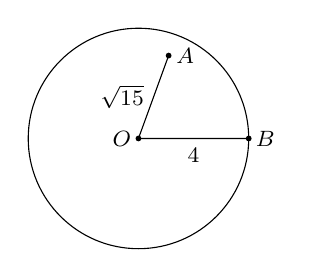
\begin{tikzpicture}[>=stealth,line join=round,line cap=round,font=\footnotesize,scale=0.7]
	\def\r{2cm}
	\path 
	(0,0) coordinate (O)
	++(0:\r)coordinate (B)
	(O)++(70:\r*0.8)coordinate (A);	
	\draw (O) circle (\r) (A)--(O)node[midway,left]{$\sqrt{15}$}--(B)node[midway,below]{$4$};	
	\foreach \m/\n in{O/180,A/0,B/0}
	\fill[black] (\m) circle(1.5pt)+(\n:3mm)node{$\m$};
	\end{tikzpicture}
	}}
\end{ex}
%%==========Câu 2
\begin{ex}
	\immini{Cho hình bên, trong đó $BD$ là đường kính, $\widehat{AOB}=40^{\circ}$; $\widehat{BOC}=100^{\circ}$. Khi đó:
	\choice
	{sđ $\wideparen{DC}=80^{\circ}$ và sđ $\wideparen{AD}=220^{\circ}$}
	{sđ $\wideparen{DC}=280^{\circ}$ và sđ $\wideparen{AD}=220^{\circ}$}
	{sđ $\wideparen{DC}=280^{\circ}$ và sđ $\wideparen{AD}=140^{\circ}$}
	{\True sđ $\wideparen{DC}=80^{\circ}$ và sđ $\wideparen{AD}=140^{\circ}$}
	}{
	\begin{tikzpicture}[>=stealth,line join=round,line cap=round,font=\footnotesize,scale=0.8]
	\def\r{2cm}
	\path 
	(0,0) coordinate (O)
	++(20:\r)coordinate (C)
	(O)++(-80:\r)coordinate (B)
	(O)++(-120:\r)coordinate (A)
	($(B)!2!(O)$) coordinate (D);	
	\draw (O) circle (\r) (D)--(B) (A)--(O)--(C);	
	\draw pic["$100^{\circ}$",angle eccentricity=1.4]{angle=B--O--C};
	\draw pic["$40^{\circ}$",angle eccentricity=2]{angle=A--O--B};
	\foreach \m/\n in{O/180,A/-120,B/-80,C/30,D/110}
	\fill[black] (\m) circle(1.5pt)+(\n:3mm)node{$\m$};
	\end{tikzpicture}}
	\loigiai{
	Vì $BD$ là đường kính nên\\
	 $\text{sđ }\wideparen{BC}+\text{sđ }\wideparen{CD}=180^{\circ}\Rightarrow \text{sđ }\wideparen{DC}=180^{\circ}-\text{sđ }\wideparen{BC}=180^{\circ}-100^{\circ}=80^{\circ}$.\\
	Vì $BD$ là đường kính nên\\
	 $\text{sđ }\wideparen{BA}+\text{sđ }\wideparen{AD}=180^{\circ}\Rightarrow \text{sđ }\wideparen{DA}=180^{\circ}-\text{sđ }\wideparen{BA}=180^{\circ}-40^{\circ}=140^{\circ}$.
	}
\end{ex}
%%==========Câu 3
\begin{ex}
	\immini{
	Trong hình bên, cho các điểm $A,B,C,D,E$ thuộc đường tròn $(O)$. Số đo góc $BOC$ là
	\choice
	{$\alpha$}
	{\True $2\alpha$}
	{$180^\circ-\alpha$}
	{$180^\circ-2\alpha$}
	}{
	\begin{tikzpicture}[font=\scriptsize, scale=.55]
	\def\r{3}
	\coordinate (O) at (0,0);
	\coordinate (A) at (110:\r);
	\coordinate (B) at (230:\r);
	\coordinate (C) at (-30:\r);
	\coordinate (D) at (10:\r);
	\coordinate (E) at (-50:\r);
	\draw (O) circle (\r);
	\draw(A)--(B)--(C)--(A)(O)--(B)--(E)(O)--(E)(B)--(D)(E)--(C)--(D);
	\draw($(A)+(-100:.3)$) arc (-100:-50:.3)node[midway, below]{$\alpha$};
	\foreach \p/\g in {A/90,B/200,C/0,D/0, E/-10, O/90}\draw[fill=black] (\p) circle (1pt)node[shift={(\g:.3)},scale=1]{$\p$};
	\end{tikzpicture}
	}
	\loigiai{
	Vì $BOC$ là góc ở tâm chắn cung $\wideparen{BC}$ nên $\widehat{BOC}=2\widehat{BAC}=2\alpha$.
	}
\end{ex}
%%==========Câu 4
\begin{ex}
	Hình quạt tròn bán kính $R$, ứng với cung $90^{\circ}$ có diện tích bằng
	\choice
	{$\pi R^2$}
	{$\dfrac{\pi R^2}{2}$}
	{\True $\dfrac{\pi R^2}{4}$}
	{$\dfrac{\pi R^2}{8}$}
	\loigiai{
	Hình quạt tròn bán kính $R$, ứng với cung $90^{\circ}$ có diện tích $S=\dfrac{\pi \cdot R^2 \cdot 90^\circ}{360}=\dfrac{\pi R^2}{4}$.
	}
\end{ex}
%%==========Câu 5
\begin{ex}
	Hình vành khuyên giới hạn bởi hai đường tròn $(O; 2\,\text{cm})$ và $(O; 4\,\text{cm})$ có diện tích bằng
	\choice
	{$12\,\text{cm}^2$}
	{$24\,\text{cm}^2$}
	{$4 \pi\,\text{cm}^2$}
	{$12 \pi\,\text{cm}^2$}
	\loigiai{
	Hình vành khuyên giới hạn bởi hai đường tròn $(O; 2\,\text{cm})$ và $(O; 4\,\text{cm})$ có diện tích
	\[S=\pi(4^2-2^2)=12\pi\,\,\text{cm}^2.\]
	}
\end{ex}
%%==========Câu 6
\begin{ex}
	Độ dài cung tròn có số đo $30^\circ$ của đường tròn bán kính $R$ là
	\choice
	{$\dfrac{\pi R}{180}$}
	{$\dfrac{\pi R}{360}$}
	{$30\pi R$}
	{\True $\dfrac{\pi R}{6}$}
	\loigiai{
	Độ dài cung tròn là $30\cdot\dfrac{\pi}{180}R=\dfrac{\pi R}{6}$.
	}
\end{ex}
%%==========Câu 7
\begin{ex}
	Diện tích của hình quạt tròn tâm $O$, bán kính $R$, cung có số đo $45^\circ$ là
	\choice
	{$\dfrac{\pi R^2}{45}$}
	{$\dfrac{\pi R^2}{4}$}
	{\True $\dfrac{\pi R^2}{8}$}
	{$\dfrac{\pi R^2}{16}$}
	\loigiai{
	Diện tích hình quạt tròn là $S=\dfrac{\pi R^2\cdot45}{360}=\dfrac{\pi R^2}{8}$.
	}
\end{ex}
%%==========Câu 8
\begin{ex}
	\immini{Cho hai đường tròn $\left(A; R_1\right)$, $\left(B; R_2\right)$, trong đó $R_2<R_1$. Biết rằng hai đường tròn $(A)$ và $(B)$ cắt nhau (H.5.44). Khi đó:
	\choice
	{$AB<R_1-R_2$}
	{\True $R_1-R_2<AB<R_1+R_2$}
	{$AB>R_1+R_2$}
	{$AB=R_1+R_2$}
	}{
	\begin{tikzpicture}[>=stealth,line join=round,line cap=round,font=\footnotesize,scale=0.35]
	\def\x{5cm}
	\def\y{4cm}
	\path 
	(0,0) coordinate (A)
	++(0:\y*1.8)coordinate (B);
	\draw[name path=c1] (A) circle (\x);
	\draw[name path=c2] (B) circle (\y);
	\path[name intersections={of= c1 and c2}] coordinate(C)at(intersection-1);
	\draw (A)--(B)--(C)node[midway,right]{$R_2$}--(A)node[midway,left]{$R_1$} ;
	\foreach \m/\n in{A/-90,B/-90,C/80}
	\fill[black] (\m) circle(1.5pt)+(\n:6mm)node{$\m$};	
	\end{tikzpicture}
	}
	\loigiai{
	Do $A$, $B$, $C$ không thẳng hàng nên $3$ điểm đó tạo thành tam giác. Áp dụng bất đẳng thức tam giác ta được\\
	 $|AC-BC|<AB<AC+BC\Rightarrow |R_1-R_2|<AB<R_1+R_2$.\\
	Mà $R_1>R_2 \Rightarrow R_1-R_2<AB<R_1+R_2 $.
	}
\end{ex}
%%==========Câu 9
\begin{ex}
	\immini{Cho đường tròn $(O; R)$; hai đường thẳng $a_1$ và $a_2$. Gọi $d_1$, $d_2$ lần lượt là khoảng cách từ điểm $O$ đến $a_1$ và $a_2$. Biết rằng $(O)$ cắt $a_1$ và tiếp xúc với $a_2$. Khi đó:
	\choice
	{\True $d_1<R$ và $d_2=R$}
	{$d_1=R$ và $d_2<R$}
	{$d_1>R$ và $d_2=R$}
	{$d_1<R$ và $d_2<R$}
	}{
	\begin{tikzpicture}[>=stealth,line join=round,line cap=round,font=\footnotesize,scale=0.8]
	\def\r{2cm}
	\path 
	(0,0) coordinate (O) node[left]{$O$}
	++(-90:\r) coordinate (H)
	(180:\r*2) coordinate (A)
	(50:\r*1.2) coordinate (B)
	(5:\r) coordinate (C)
	($(A)!(O)!(B)$)coordinate (K)
	(-2*\r,-\r) coordinate (E);
	\draw 
	(O) circle (\r) 
	(O)--(H) node[midway, right]{$d_2$}
	(O)--(K) node[midway, right]{$d_1$}
	(O)--(C) node[midway, above]{$R$}
	(A)node[above right]{$a_1$}--(B)
	(E)node[above right]{$a_2$}--(1.2*\r,-\r) ;
	\draw pic[draw,angle radius=0.2cm]{right angle=A--K--O};
	\draw pic[draw,angle radius=0.2cm]{right angle=O--H--E};	
	\end{tikzpicture}
	}
	\loigiai{
	\immini{
	Gọi $H$, $K$ là chân đường vuông góc lần lượt hạ từ $O$ đến $a_1$ và $a_2$.\\
	\begin{itemize}
	\item Ta có $d_1=OK$, mà $K$ nằm trong đường tròn nên $OK<R\Rightarrow d_1<R.$
	\item Ta có $d_2=OH$, mà $H$ nằm trên đường tròn nên $OH=R\Rightarrow d_2=R.$
	\end{itemize}}{
	\begin{tikzpicture}[>=stealth,line join=round,line cap=round,font=\footnotesize,scale=0.8]
	\def\r{2cm}
	\path 
	(0,0) coordinate (O) node[left]{$O$}
	++(-90:\r) coordinate (H) node[below]{$H$}
	(180:\r*2) coordinate (A)
	(50:\r*1.2) coordinate (B)
	(5:\r) coordinate (C)
	($(A)!(O)!(B)$)coordinate (K)node[above left]{$K$}
	(-2*\r,-\r) coordinate (E);
	\draw 
	(O) circle (\r) 
	(O)--(H) node[midway, right]{$d_2$}
	(O)--(K) node[midway, right]{$d_1$}
	(O)--(C) node[midway, above]{$R$}
	(A)node[above right]{$a_1$}--(B)
	(E)node[above right]{$a_2$}--(1.2*\r,-\r) ;
	\draw pic[draw,angle radius=0.2cm]{right angle=A--K--O};
	\draw pic[draw,angle radius=0.2cm]{right angle=O--H--E};	
	\end{tikzpicture}
	}
	}
\end{ex}
%%==========Câu 10
\begin{ex}
	Cho hai đường tròn $(O;5\,\text{cm})$, $\left(O'; 4\,\text{cm}\right)$ với $OO'=9\,\text{cm}$. Kết luận nào sau đây đúng về vị trí tương đối của hai đường tròn?
	\choice
	{Hai đường tròn cắt nhau}
	{Hai đường tròn ở ngoài nhau}
	{\True Hai đường tròn tiếp xúc ngoài}
	{Hai đường tròn tiếp xúc trong}
	\loigiai{
	Đường tròn $(O)$ có bán kính $R=5$ cm và đường tròn $(O')$ có bán kính $R'=4$ cm.\\
	Ta thấy $R+R'=5+4=9\,\,\text{cm}=OO'$. Do đó hai đường tròn tiếp xúc ngoài.
	}
\end{ex}
%%==========Câu 11
\begin{ex}
	Cho đường tròn $(0; 6\,\text{cm})$ và đường thẳng $a$ với khoảng cách từ $O$ đến $a$ là $4\,\text{cm}$. Kết luận nào sau đây đúng về vi trí giữa đường tròn $(O)$ và đường thẳng $a$?
	\choice
	{\True $(O)$ và $a$ cắt nhau tại hai điểm}
	{$(O)$ và $a$ tiếp xúc}
	{$(O)$ và $a$ không có điểm chung}
	{$(O)$ và $a$ có duy nhất điểm chung}
	\loigiai{
	Ta thấy khoảng cách từ $O$ đến đường thẳng $a$ là $4$ cm nhỏ hơn bán kính của đường tròn $(O)$ ($6$ cm) nên đường tròn $(O)$ cắt đường thẳng $a$ tại hai điểm.
	}
\end{ex}
%%==========Câu 12
\begin{ex}
	Góc ở tâm là góc
	\choice
	{\True có đỉnh nằm trên đường tròn}
	{có đỉnh nằm trên bán kính của đường tròn}
	{có hai cạnh là hai đường kính của đường tròn}
	{có đỉnh trùng với tâm đường tròn}
	\loigiai{
	Theo định nghĩa thì góc ở tâm là góc có đỉnh nằm trên đường tròn.
	}
\end{ex}
%%==========Câu 13
\begin{ex}
	\immini{
	Cho hai tiếp tuyến của đường tròn $(O)$ tại $A$ và $B$ cắt nhau tại $M$ (hình bên). Biết $\widehat{AMB}=50^{\circ}$. Số đo cung nhỏ $AB$ là
	\choice
	{$140^{\circ}$}
	{$230^{\circ}$}
	{\True $130^{\circ}$}
	{$150^{\circ}$}	
	}{
	\begin{tikzpicture}[>=stealth,line join=round,line cap=round,font=\footnotesize,scale=1]
	\tikzset{declare function={r=1.5;r2=r/sin(25);}}
	\draw[name path=circleO] (0,0)coordinate (O) circle (r);
	\path 
	($(O)+(0:r*2.2)$)coordinate (M)
	;
	% Vẽ tiếp tuyến
	\path[name path=circleX] let \p1=($(O)-($(O)!.5!(M)$)$) in ($(O)!.5!(M)$) circle ({veclen(\x1,\y1)});
	\path[name intersections={of= circleX and circleO}] coordinate (A) at (intersection-1) coordinate (B) at (intersection-2);
	\path 
	pic[draw,angle radius=2mm]{right angle=O--B--M}
	pic[draw,angle radius=2mm]{right angle=O--A--M}
	pic[draw,angle radius=2mm]{angle=A--M--O}
	pic[draw,angle radius=2.3mm]{angle=O--M--B}
	;
	\foreach \pointo/\pointt in {O/A,O/B,O/M,A/B,M/A,M/B}{
	\draw[fill=black](\pointo)--(\pointt);
	}
	\foreach \point/\goc in {O/180,M/0,B/-60,A/60}{
	\draw[fill=black](\point)circle(.8pt)+(\goc:2mm)node[scale=.8]{$\point$};
	}
	\end{tikzpicture}
	}
	\loigiai{
	Tứ giác $AOBM$ có $\widehat{AOB}=360^{\circ}-\widehat{MAO}-\widehat{MBO}-\widehat{AMB}=360^{\circ}-90^{\circ}-90^{\circ}-50^{\circ}=130^{\circ}$.\\
	Khi đó $\text{sđ}\wideparen{AB}=\widehat{AOB}=130^{\circ}$.
	}
\end{ex}
\Closesolutionfile{ans}
%%%%%%%%%%%%%